\subsection{\label{sec:photonic_neural_systems}Photonic Neural Systems}
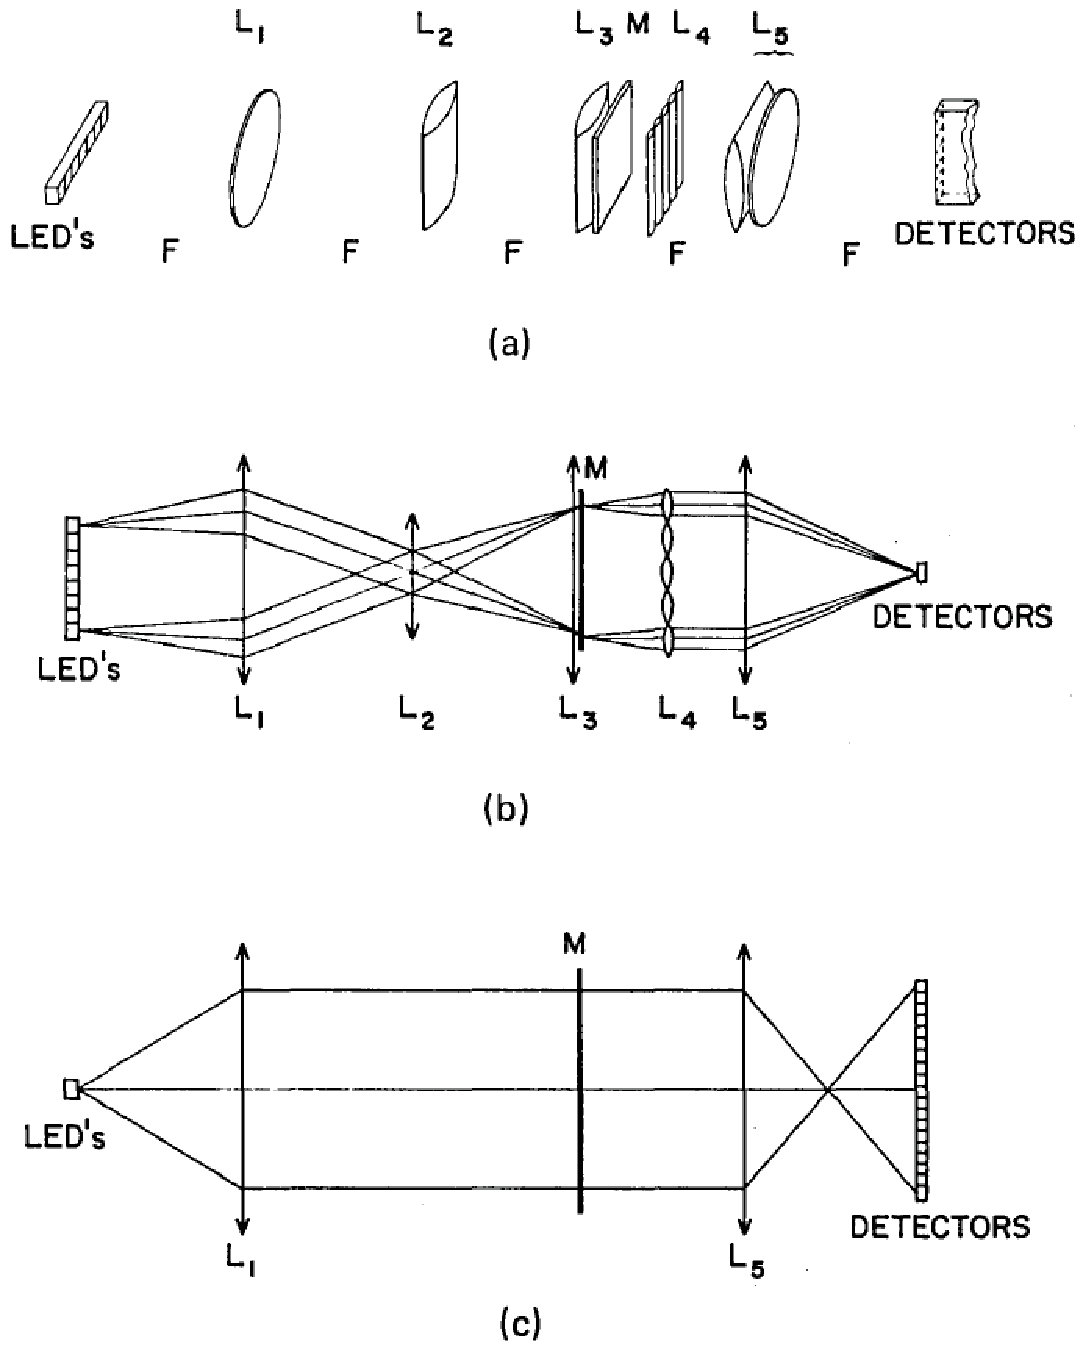
\includegraphics[width=8.6cm]{figures/_stanford_architecture.pdf}
\captionof{figure}{\label{fig:stanford_architecture}The Stanford architecture for optical matrix-vector multiplication. (a) Pictorial view; (b) top view; (c) side view. From Ref.\,\onlinecite{godi1978}.\vspace{1em}}
The strengths of optics in computing have been acknowledged for decades and have led to many attempts to design digital computing architectures around optical phenomena and devices. Like AI and superconductors, there have been several waves interest in photonics for computing. The first wave of interest began in the late 1970s and was triggered by the seminal paper from Goodman, Dias, and Woody regarding the use of optics for performing Fourier transforms with incoherent light \cite{godi1978}. This work generated a great deal of interest because it showed the power of optics for performing matrix-vector multiplication with complex quantities in a parallel manner using incoherent light that does not have phase as an accessible parameter. The concept is shown in Fig.\,\ref{fig:stanford_architecture}. A primary favorable feature of optical matrix-vector multiplication is that the time required for the operation is, in principle, nearly independent of the dimension of matrix. This is in contrast to a quadratic temporal scaling with conventional digital approaches. While other Fourier transform devices had been proposed, including in slab-guided modes in integrated photonic systems \cite{shha1968,anbo1977}, the work by Goodman, Dias, and Woody combined several key ideas at the right time to generate significant excitement around the use of optics in computing. The optical approach to matrix-vector multiplication introduced in Ref.\,\onlinecite{godi1978} is now referred to as the \textit{Stanford architecture}, as the authors were working at Stanford University at the time of the publication.

Themes raised in the Stanford architecture persist to the present. The primary theme is the use of light for highly parallel computation. Each light source can straightforwardly fan its signal out along many optical paths, and parallel computation can occur along each path independently. More generally, the primary strength of optics lies in communication\textemdash the ability to rapidly move information from one place to another without degradation. This strength is fundamental to the uncharged, massless, bosonic nature of photons which allows them to propagate without interaction. This strength is utilized from kHz and MHz frequencies for radio communication up to hundreds of THz for intercontinental data transmission over optical fiber.

Another theme raised by the Stanford Architecture is the use of optics for special-purpose hardware accelerators that perform a specific task with performance unmatched by electronic approaches. Goodman et al. focused on the Fourier transform, but matrix-vector multiplication is the underlying operation. The non-interacting nature of light makes it excellent for parallel data transmission, which enables efficient matrix-vector multiplication. However, to construct a general purpose computer in the model of Turing, nonlinear operations are necessary. Efforts to augment the strength of light for communication with nonlinear optical devices for \textit{all-optical} computing surged in the 1980s following the work of Goodman, Dias, and Woody. These efforts can be separated roughly into two categories, with one track being focused on displacing silicon electronics for digital logic and general-purpose computing, and another track maintaining the purpose of augmenting silicon electronics with task-specific hardware accelerators that were envisioned to work in conjunction with electronic digital computers. The introduction of the Stanford architecture was shortly followed by a wave of interest in neural networks, and the use of optics for neural networks based on a similar architecture was quickly introduced \cite{psfa1985}.

In the following subsection, we briefly review efforts to utilize light in digital computing from the 1970s until the present to establish the context for the evolution of photonic neural systems.

\subsubsection{Optical Logic Elements}
As stated above, the strengths of optics for information processing have been known for some time and have inspired many efforts to conceive of and construct systems for all-optical computing as well as hybrid optoelectronic architectures. The primary strengths of light for information processing are the potential for massive fan out and parallelism, low latency, and high bandwidth. These attributes motivated the Stanford architecture as well as a great deal of other research. The weakness of optics for information processing is that precisely the same as its strength: because photons are uncharged bosons, they do not interact, and therefore they do not have nonlinear responses, and are therefore limited in the input-output transfer functions they can instantiate for computation. Efforts to leverage the strengths of optics for computing have paid significant attention to techniques and devices to give rise to optical nonlinearities that can be leveraged for digital logic gates.

Devices demonstrating optical bistability have been a primary direction of research to enable optical devices that can be used to construct logic gates. The state of the field was reviewed comprehensively in 1982 by Abraham and Smith \cite{abms1982}, and the authors summarize the subject: ``Optical bistability is a general title for a number of static and dynamic phenomena that result from the interplay of optical non-linearity and feedback.'' The 1985 book by Gibbs also summarizes the field at that time \cite{gi1985}. The primary goals of optical bistable devices are to construct optical transistors and optical memory elements. An optical transistor is a device wherein one optical beam controls the propagation of another optical beam. Optical memory is most often implemented by using an optical signal to change the state of a solid-state element, which can then be interrogated optically. It is essentially impossible to induce light to halt its motion, and it is difficult to extend the decay lifetime of photons propagating within a cavity beyond the nanosecond scale, so optical memory based on the storage of photons in a particular location is not feasible.

The first demonstration of optical bistability was achieved by Gibbs, McCall, and Venkatesan in 1976 \cite{gimc1976}. The physical system achieving the bistability comprised a Fabry-Perot interferometer filled with sodium vapor. The sodium vapor provided a nonlinear dispersive medium so that the transmitted intensity was a nonlinear function of the incident intensity. Miller, Smith, and Johnston leveraged a similar effect in a Fabry-Perot cavity formed from an InSb crystal in 1979 \cite{mism1979}. In this work, the nonlinear refraction was based on electronic nonlinearity related to states below the semiconductor band gap, and the use of a semiconductor crystal rather than an atomic vapor made the system more likely to be useful in complex computing systems. Reference \onlinecite{mism1979} demonstrated optical differential gain and bistability. Because the system enabled a weak beam to modulate the transmission of a powerful beam, this system provided the first example of an optical transistor. The overall small signal power gain was greater than six. Subsequent work integrated devices leveraging this principle as a 2D array of etalons \cite{jele1986,vewi1986} for the purpose of performing logical operations. 

An alternative approach to bistable optical devices was based on the self-electrooptic effect device. Work on self-electrooptic devices was also carried out by Miller, beginning in 1984 \cite{mich1984}. The principle of operation is based on adjustable absorption controlled with an electric field applied perpendicular to the plane of the quantum well that shifts the band edge, known as the quantum confined Stark effect \cite{mich1984b}. In a self-electrooptic effect device, the quantum confined Stark effect as well as optical detection are present in a single structure, leading to optoelectronic feedback that produces bistability. A number of configurations of such devices have been implemented, with the symmetric self-electrooptic effect device introduced by Lentine et al. being the most successful \cite{lehi1988,lehi1989}. In this implementation, two $p$-$i$-$n$ diodes with quantum wells in the intrinsic regions are combined, each serving as the load for the other. As Lentine states, ``This device has complimentary outputs whose switching point is determined by the ratio of the two optical input powers and acts as a set-reset latch.'' One strength of this device is that it has time-sequential gain, meaning once set with low-power beams, it can be subsequently read out with high-power beams. This results in good input-output isolation because the large output occurs at a later time than the inputs. Additionally, while previous electrooptical devices with optical bistability required critical biasing very close to a nonlinear threshold, no such biasing was required.

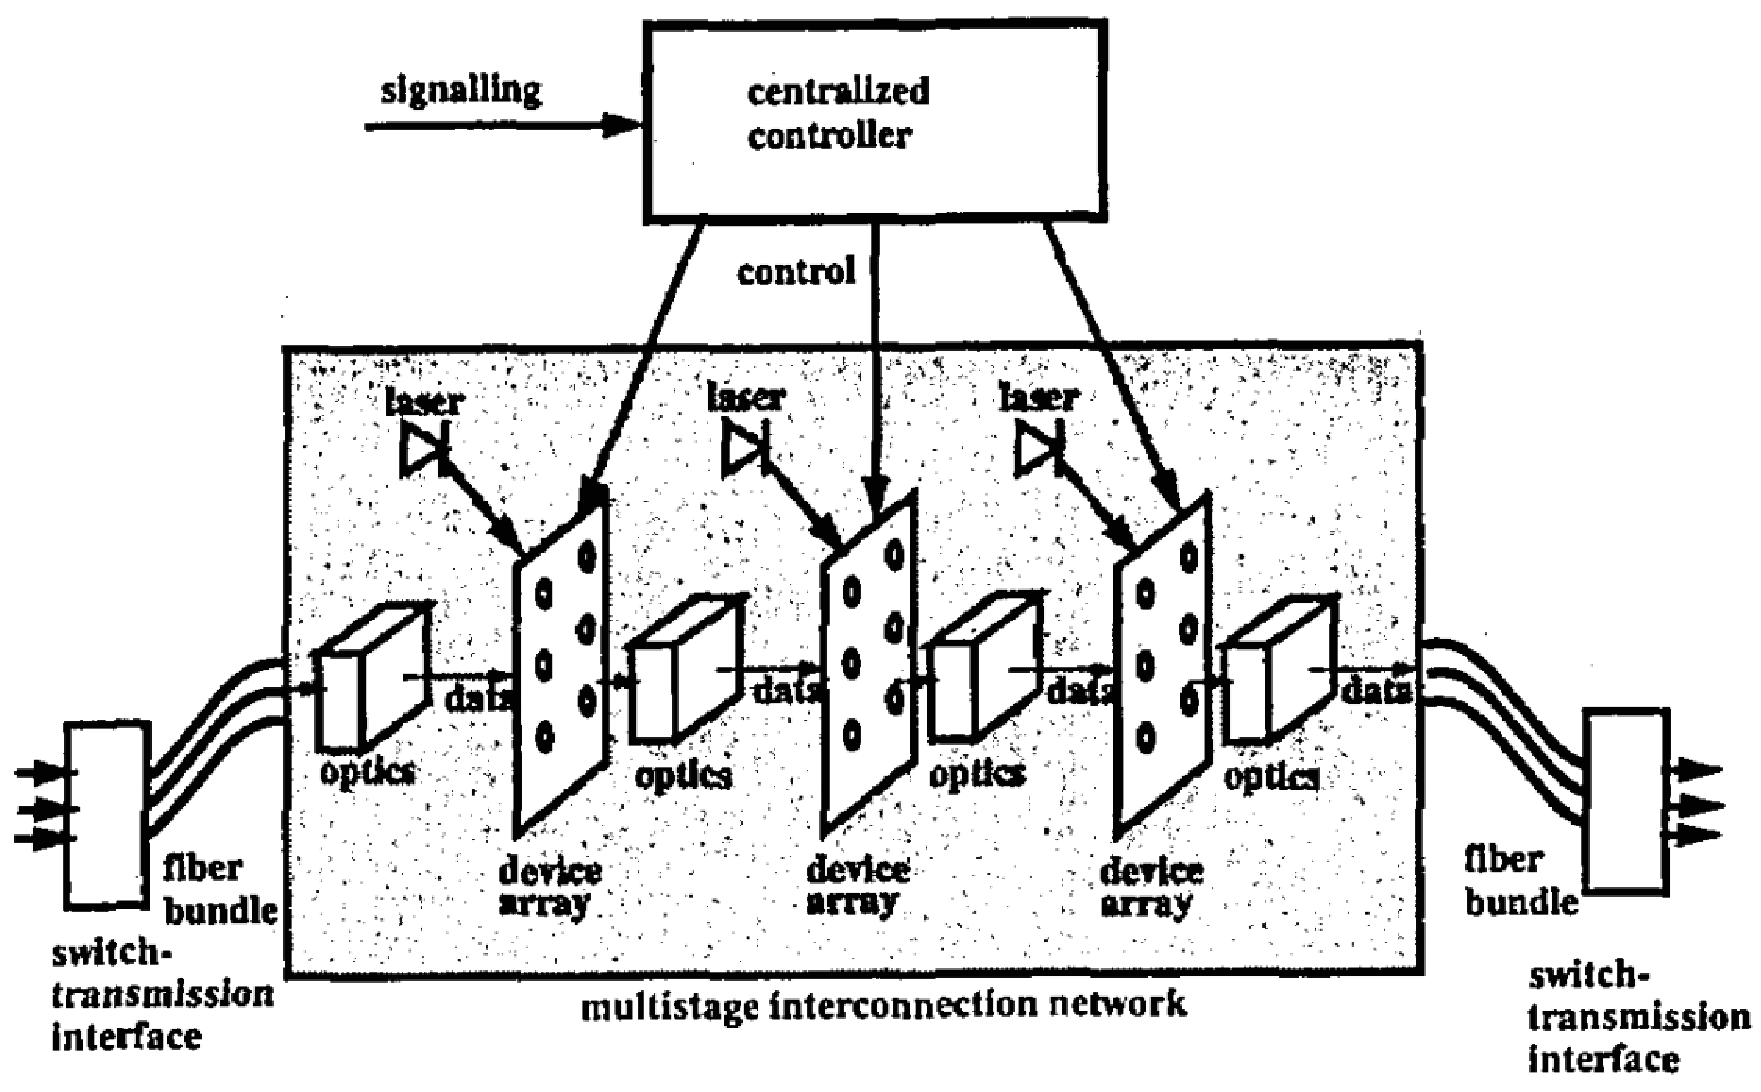
\includegraphics[width=8.6cm]{figures/_optical_switching_network.pdf}
\captionof{figure}{\label{fig:optical_switching_network}Centrally controlled free-space photonic switching fabric. From Ref.\,\onlinecite{mccl1993}.\vspace{1em}}
A switching network comprised of symmetric self-electrooptic-effect devices was demonstrated by McCormick et al. in 1993 \cite{mccl1993}. This free-space optical system comprised a 32$\times$32 switching node array of these devices. Light propagated perpendicular to the plane of the device array, and 16 input channels were connected to 32 output channels with each channel transmitting 32 bits in parallel. The input data to be routed entered on optical fibers and was coupled to free space. Six stages of electrooptic devices were present, each with input control lasers, electronic control through an electronic computer, and with optics between the stages. The output was again coupled to fibers.

Other approaches to the creation of optical transistors have continued to be proposed as nanoscale patterning of photonic devices has become commonplace. One example is the design of an optical transistor based on a photonic crystal cavity \cite{yafa2003} that was presented in 2003 by Yanik, Fan, Solja\v{c}i\'{c}, and Joannopoulos. In this on-chip structure, two waveguides lead into a photonic crystal cavity, and two waveguides lead out. In this case, the photonic crystal cavity plays the role of the Fabry-Perot utilized by Miller et al., and a control beam input into one of the inputs shifts the resonance of the cavity through the Kerr nonlinearity. With this beam present, transmission of the signal beam is high, while without the control beam, transmission of the signal beam is low. The authors simulated this operation with material parameters corresponding to AlGaAs, and found that with a modest $Q$ factor of 5000, the contrast ratio between on and off states could be as high as 10 with a few milliwatts of input power. 

Another optical transistor leveraging nano-scale optical phenomena is based on switching a single molecule between internal electronic states and has been demonstrated by Sandoghdar's group in 2009 \cite{hwpo2009}. Other recent efforts to realize bistable optical devices for computing and telecommunications include the use of graphene \cite{wawu2016,guru2017}, semiconductor quantum wells \cite{suzh2019,saeb2018}, and semiconductor quantum dots \cite{lili2019}. 

After 40 years of effort in optical logic devices, no candidate looks promising to displace the electronic transistor for large-scale digital computing. As Miller stated in 2010, ``Only one device has apparently ever satisfied [the success] criteria well enough to allow large logic systems to be constructed.'' \cite{mi2010} Miller was referring to the self-electrooptic-effect devices of Lentine \cite{lehi1989} and the switching systems of McCormick \cite{mccl1993}. Difficulties with optical logic devices do not mean the field of photonics has stalled in the past several decades. To the contrary, tremendous progress has been made. Much of this progress has been enabled by the birth of silicon photonics. Let us put this discussion of optical logic devices to the side while we discuss integrated silicon photonics. Then we will attempt to synthesize what the past 40 year of research in optical technologies can teach us regarding the design of hardware for cognitive systems.

%Based on this brief summary of optical logic devices, can we identify common trends that can guide future thinking on the use of optics in computing in general and for cognitive hardware in particular?

\subsubsection{\label{sec:integrated_silicon_photonics}Integrated Silicon Photonics}

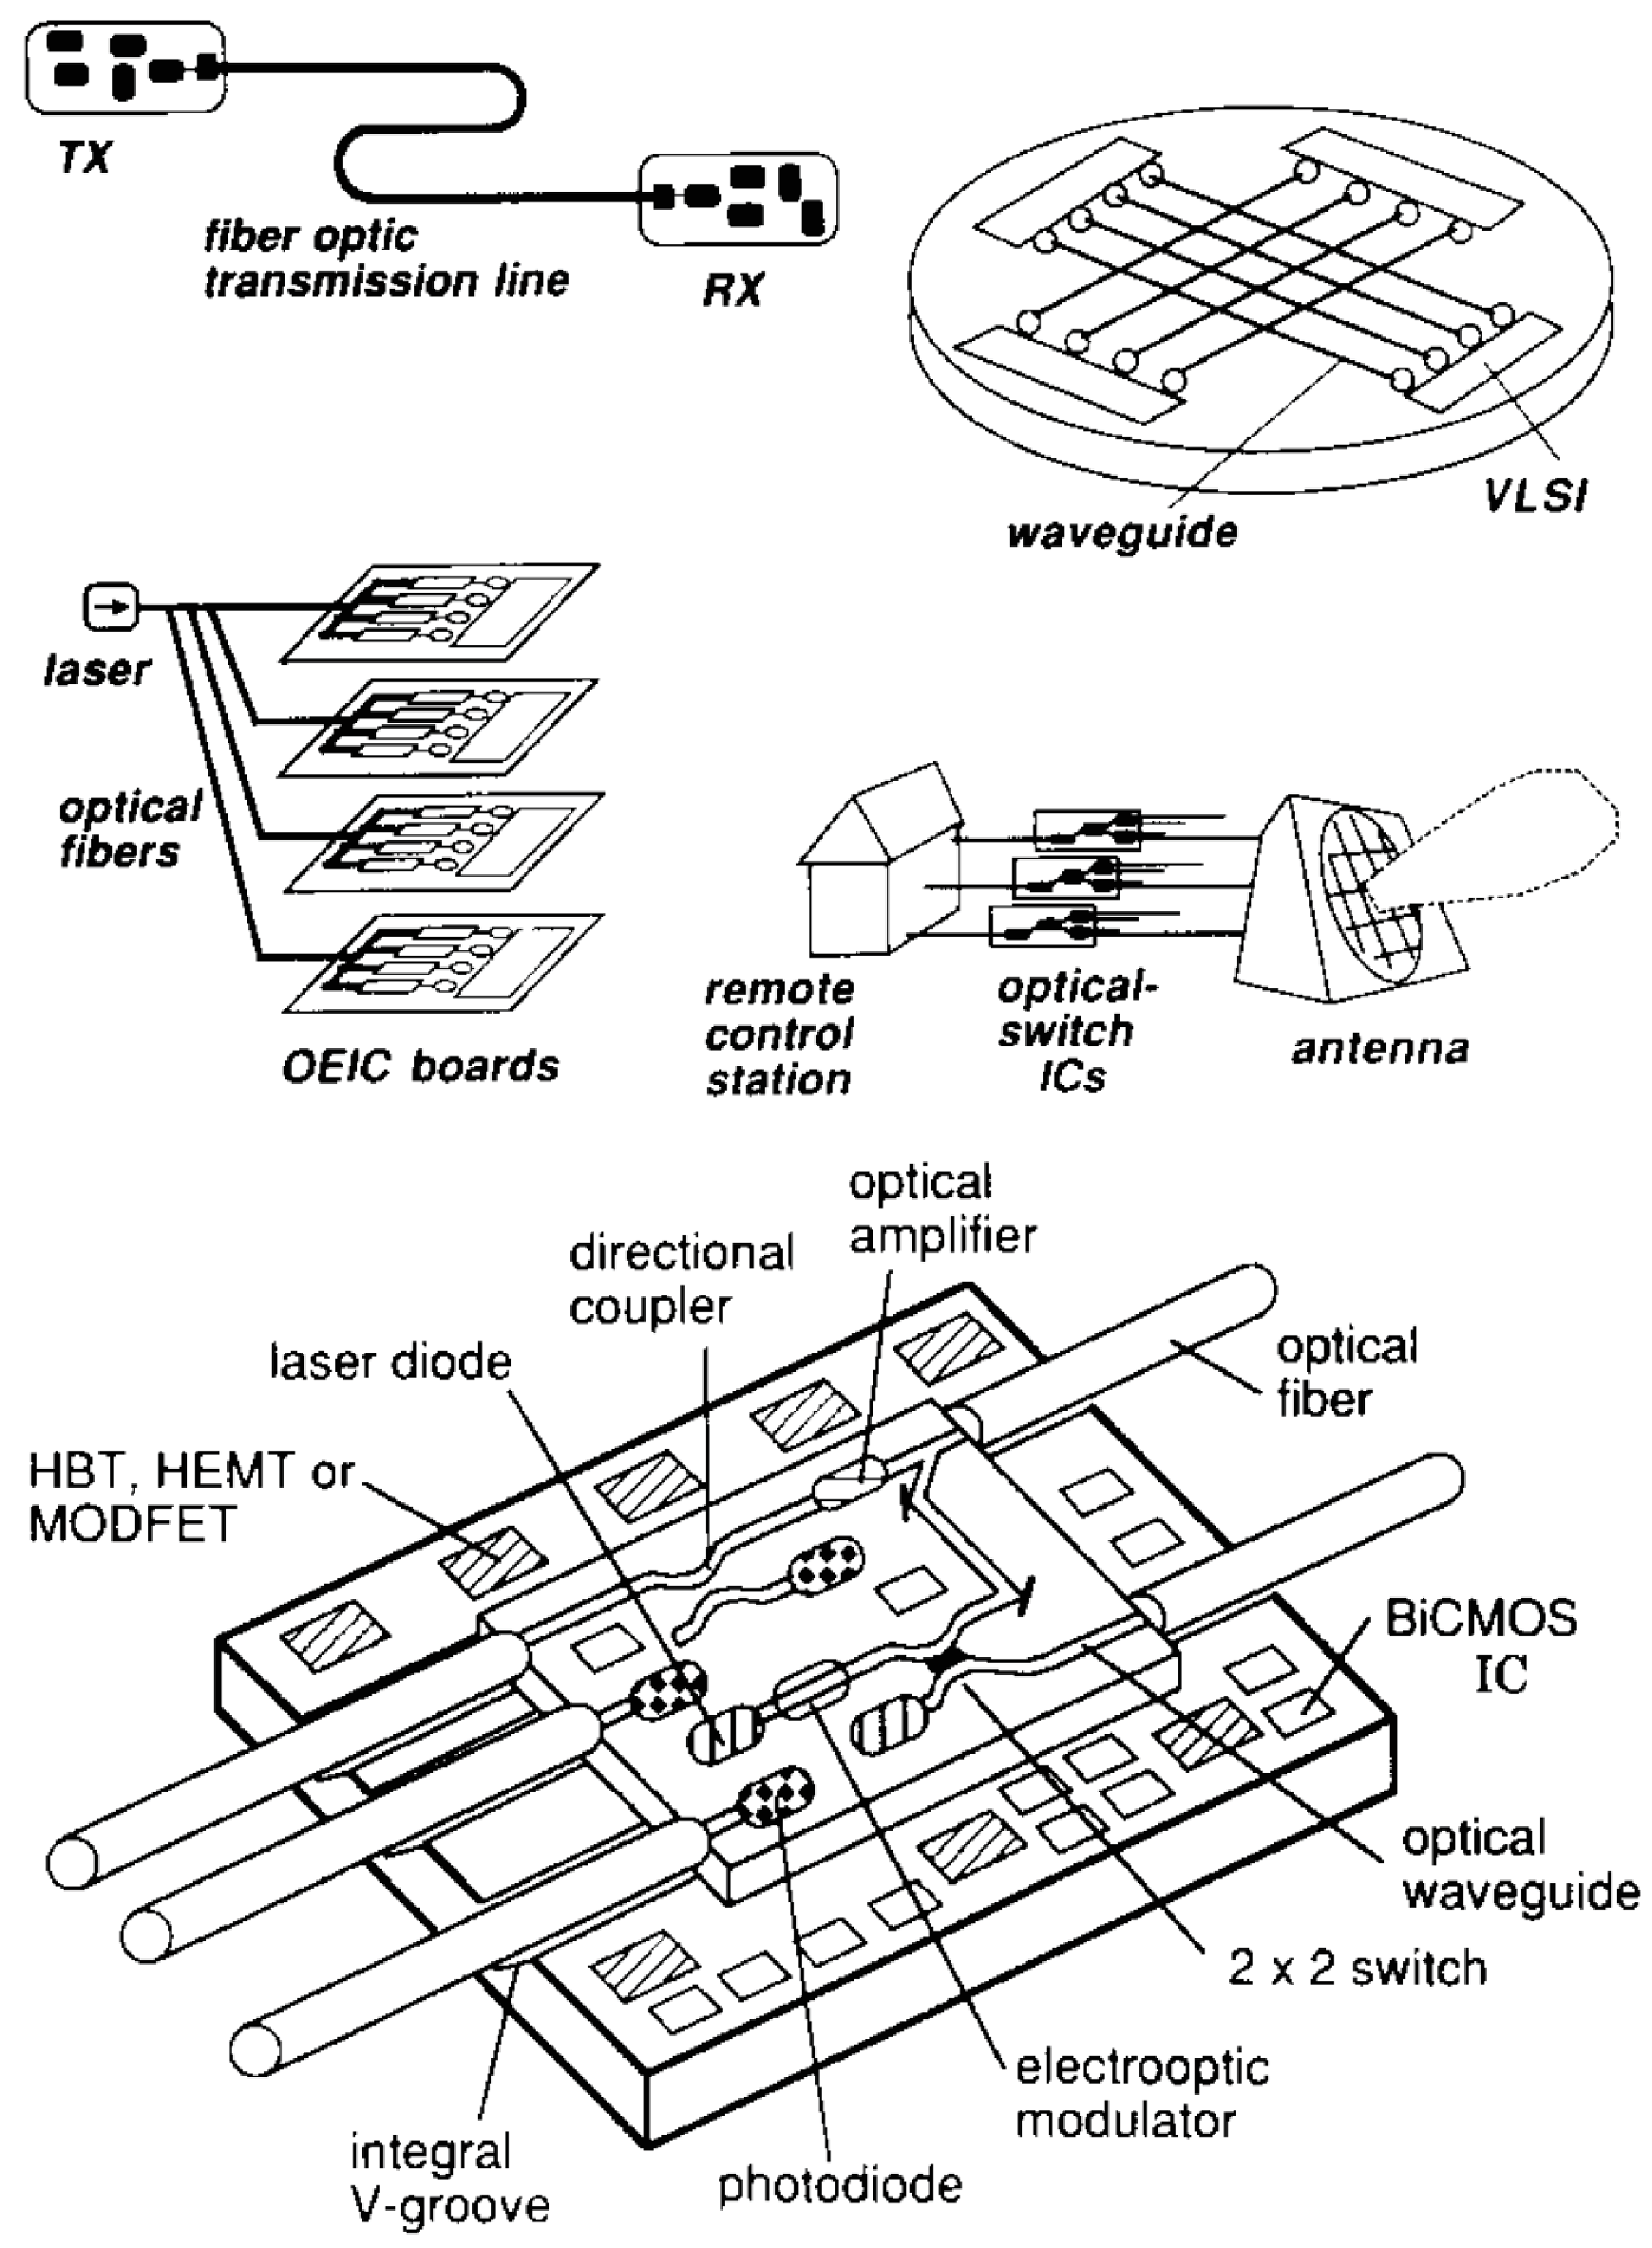
\includegraphics[width=8.6cm]{figures/_soref_1993.pdf}
\captionof{figure}{\label{fig:soref_1993}Richard Soref's vision of superchips. From Ref.\,\onlinecite{so1993}.\vspace{1em}}
By the mid 1980s, silicon microelectronics was well established as the supreme technology for computing. The scaling predictions made by Moore in 1965 \cite{mo1965} had held for two decades, while other material platforms for electronics and photonics had not met with the same success. Within this context, a new perspective on the role of light in computing was put forward in a series of papers by Soref, Lorenzo, and Bennett from 1985 to 1987 \cite{sole1985,sole1986,sobe1987}. The state of the field was reviewed by Soref in 1993 in Ref.\,\cite{so1993}, in which he states that the ``impetus for investigating silicon photonics comes mainly from the vision of optoelectronics: the integration of optics and electronics on the same substrate.'' Soref anticipated that the resulting ``superchips'' would ``have performance and functionality greater than those of the optical and electrical circuits taken alone.'' Soref's concept of superchips are illustrated in Fig.\,\ref{fig:soref_1993}. While other materials (primarily compound semiconductors) had been developed for integrated optical components prior to the work by Soref et al., this series of papers pointed to the potential for integrated optical components to be incorporated with silicon microelectronics monolithically. As the authors stated, ``Silicon is a `new' material in the context of integrated optics even though Si is the most thoroughly studied semiconductor in the world. There is reason to believe that Si can serve as the medium for a variety of guided-wave optical components in much the same manner as III-V semiconductor compounds, while at the same time avoiding the inherent complexities of binary, ternary, and quarternary alloys.'' \cite{sole1986} They further describe their two primary motivations: 1) to utilize the fabrication processes that have been developed for the Si electronic circuit industry in the production of photonic devices; and 2) to monolithically combine silicon electronic circuits with guided-wave optoelectronic components. The goal was to follow the model of the integrated circuit that had become tremendously successful by the mid 1980s. This model utilizes lithographic fabrication to realize system complexity that can be achieved only through integration of components on a chip.

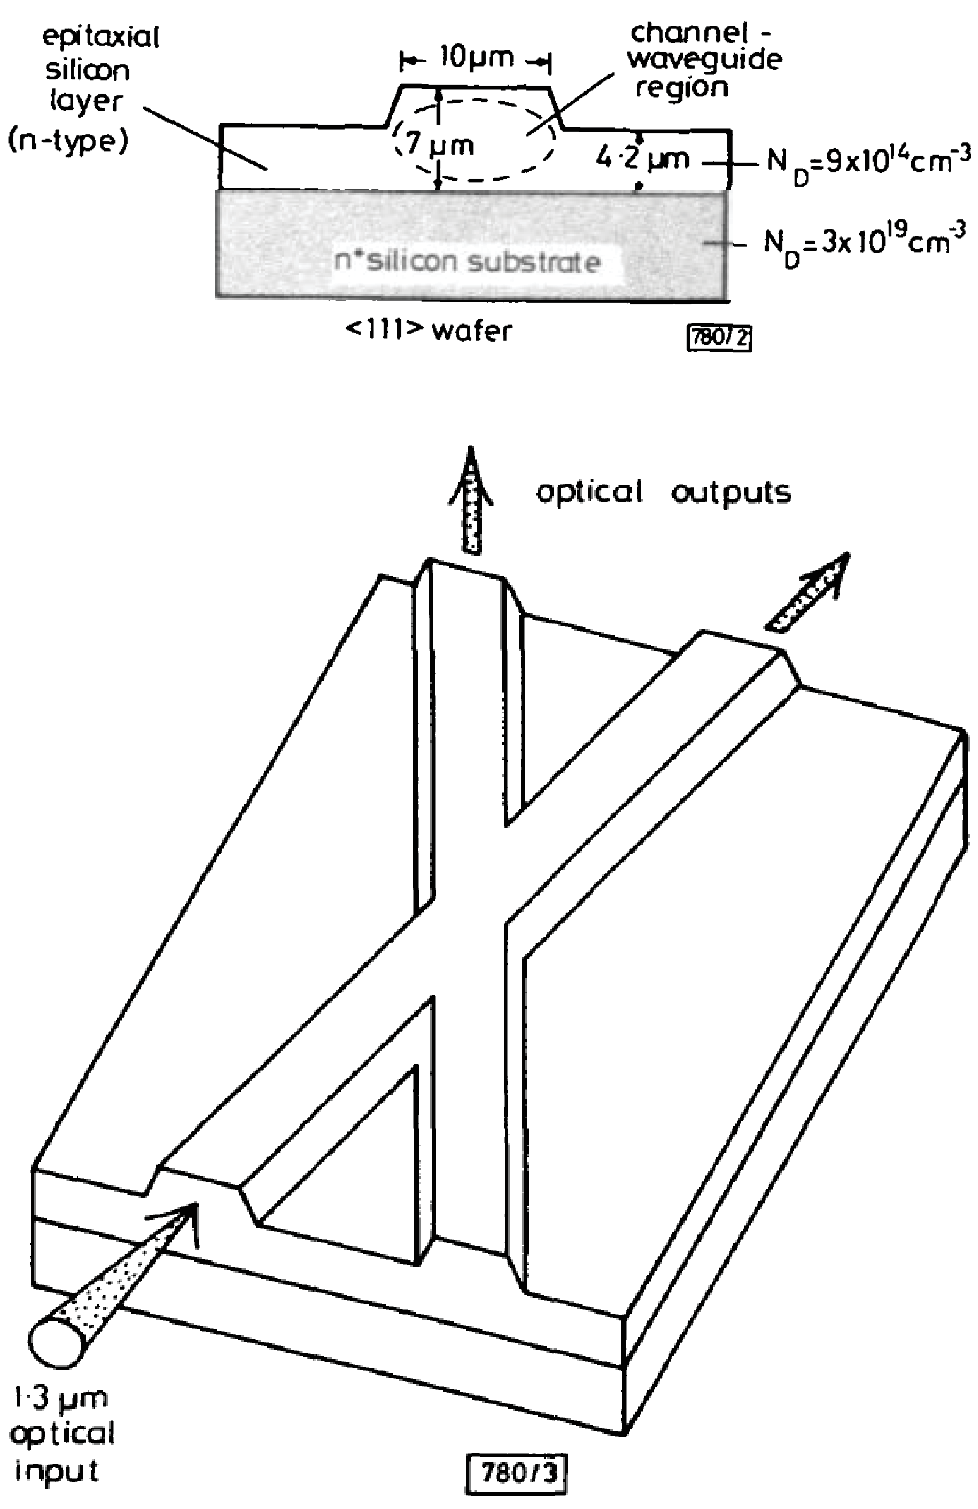
\includegraphics[width=8.6cm]{figures/_soref_1985.pdf}
\captionof{figure}{\label{fig:soref_1985}Schematic of the first silicon photonic waveguide. From Ref.\,\onlinecite{sole1985}.\vspace{1em}}
In the first paper of the series, passive waveguides and power dividers were demonstrated at $\lambda = 1.3$\,\textmu m, a wavelength at which optical fibers are highly transmissive, indiciating the potential for silicon photonic components to interface with both electronic computational infrastructure as well as fiber-optic communication infrastructure. Optical confinement was achieved in the vertical dimension by epitaxially growing intrinsic silicon on a heavily $n$-type doped silicon substrate, which has a slightly lower index of refraction \footnote{The index change due to free carriers can be calculated with the classical dispersion formula given in Ref.\,\cite{sole1985}: $\Delta n = -(e^2\lambda^2/8\pi^2 c^2n\epsilon_0)(\Delta N_em_{ce}^*+\Delta N_hm_{ch}^*]$, where $e$ is the charge of an electron, $\lambda$ is the optical wavelength, $n$ is the refractive index of the intrinsic material, $\epsilon_0$ is the permittivity of free space, $c$ is the velocity of light in vacuum, $N_e$ ($N_h$) is the concentration of donors (acceptors), and $m_ce^*$ ($m_ch^*$) is the effective mass of electrons (holes).}. In the lateral dimension, confinement was achieved by etching a fraction of the depth of the epitaxial intrinsic silicon, leading to a so-called rib waveguide configuration \footnote{A rib waveguide results from partial etching of the high-index layer, while a ridge waveguide results from etching completely through the high-index layer. Foundations of optical waveguide theory can be found in Refs.\,\cite{snlo1983} and \cite{hu2009}.}. The waveguide structure is shown in Fig.\,\ref{fig:soref_waveguide}(a). The passive power splitter is shown in Fig.\,\ref{fig:soref_waveguide}(b). These are the first silicon photonic components.

In the second paper on the subject, Soref and Lorenzo describe active silicon photonic components based on free-carrier dispersion effects \cite{solo1986}. Because the silicon lattice is centrosymmetric, a linear electrooptic effect is not present in bulk crystals, and therefore many had not considered silicon a candidate for active optical components. The insight by Soref and Lorenzo to utilize free-carrier effects instead opened many opportunites that would lead to over three decades of technology development. In Ref.\,\onlinecite{solo1986}, silicon-germanium compounds were also proposed as complimentary materials for waveguiding, and silicon-on-insulator (SOI) structures were considered as candidates for a layer structure capable of optical confinement.

A subsequent paper by Soref and Bennett theoretically analyzed the index perturbation achieved by injecting charges or depleting them from silicon \cite{sobe1987}. This work had a tremendous impact because it made the case that active components such as modulators and switches could be created in silicon by shifting the phase of light propagating through an interferometer or resonator. Soref and Bennett showed that a sufficient phase shift could be induced to produce a useful active device without incurring intolerable free-carrier absorption. Essentially all present-day silicon modulators are based on these free-carrier effects.

At the time of the original work by Soref et al., SOI technologies were just beginning to be developed, and epitaxial intrinsic silicon grown on heavily doped silicon gave the best waveguiding results. As silicon-on-insulator technology improved\textemdash particularly through device-layer transfer rather than epitaxial growith\textemdash the situation changed dramatically. The ability to fabricate a thin layer of intrinsic crystalline silicon on top of an electrically insulating layer with lower index of refraction has proved consequential for both electronic and photonic devices. The basic layer structure of SOI is shown in Fig.\,\ref{fig:soi}. In particular, the properties of the Si/SiO$_2$ interface are crucial for enabling low-loss SOI waveguides. Just as the physical and chemical properties of SiO$_2$ and the interface with Si were one of the primary factors that led to silicon being the most successful material for VLSI electronics (see Sec.\,\ref{sec:general_hardware_considerations}), these basic material properties are central to the success of silicon photonics, as will be discussed below.

The ideas of Soref, Lorenzo, and Bennett pointed to the potential for exciting integrated photonic devices based on silicon, but the field of silicon photonics did not launch in earnest until SOI technology became mature. Around the year 2000, SOI technology had improved to the point where major semiconductor manufacturers were using SOI wafers for the production of high-performance transistors. This shift was motivated by performance enhancements such as the higher speed at the same supply voltage, or lower voltage and therefore lower power consumption at the same speed as previous technology generations \cite{cecr2003}. As transistor gate lengths continued to decrease, the carrier confinement provided by a thin device layer on top of an insulator became necessary to reduce short channel effects.

Early silicon electrooptic modulators utilizing charge-carrier effects outlined by Soref, Lorenzo, and Bennett emerged in 2004 as SOI with thicker buried oxide for photonic confinement became commercially available. These employed MOS capacitor designs \cite{lijo2004,lisa2005} as well as and microring-based \cite{xusc2005,xuma2007} $p$-$i$-$n$ carrier-injection designs to reach data rates in the Gbps range. Significant progress occurred rapidly due to the ability to leverage existing silicon manufacturing techniques. The state of the field of silicon electrooptic modulators was reviewed in 2010 by Reed et al. \cite{rema2010} and more recently by Witzens \cite{wi2018}, with data rates of modulators employing charge-carrier effects now in in the range of 50\,Gbps \cite{pasa2015}. 

In 1993, Soref wrote, ``The decade of the 1990's is an opportune time for scientists and engineers to create cost-effective silicon `superchips' that merge silicon photonics with advanced silicon electronics on a silicon substrate.'' Has Soref's vision of the superchip come to fruition? Passive and active silicon photonic devices have affected an astonishing range of application spaces, from medical diagnostics to telecommunications, but the computing industry has not yet been dramatically transformed by silicon photonics. Silicon transceivers are becoming commonplace in data centers, but primarily as separate modules for interconnection between server racks. Multiple silicon photonic foundries exist throughout the world, confirming Soref's expectation that silicon photonics would benefit from knowledge gained by the silicon electronics industry. The accomplishment that comes closest to the superchip has leveraged the ``zero-change'' approach to electronic-photonic integration. The principle is to produce photonic components in a CMOS process with no changes to the process itself. Because any CMOS process is finely tuned to achieve high transistor performance, any attempt to introduce changes to the process to accommodate photonic devices will degrade the performance of electronics and significantly increase cost. To insert photonic components into the computing ecosystem in an economically viable manner, minimal disruption is required. Following this model, it has been shown that many passive and active components can be manufactured in a 45-nm CMOS foundry by utilizing the crystalline silicon layer of an SOI wafer that is intended to be used for transistor to produce waveguides as well \cite{orma2012}. Using dopants already present in the process for transistor fabrication, it has been shown that modulators can be fabricated \cite{shor2013,alch2016}. With a similar cavity and doping configuration, and using the SiGe that is incorporated in the process for strain engineering of transistors, photodetectors have been demonstrated \cite{alra2016}. Similar components have been demonstrated in a lower-cost polycrystalline bulk CMOS process \cite{shor2013b,meor2014}. 

The monolithic integration of high-performance CMOS electronics with silicon photonics was used to demonstrate an electrooptic system on a chip combining a processor and random-access memory where the only communication from the chip to the outside was through optical signals generated by on-chip modulators driven by the CMOS electronics \cite{suwa2015}. Using two such chips, the project demonstrated direct optical chip-to-chip communication to build a photonically connected main memory system for the microprocessor. The microprocessor communicated to the memory on the other chip, and memory-intensive applications were demonstrated using only this optical processor-to-memory link \cite{suwa2015}. The state of the field of zero-change photonic-electronic integration was reviewed by Stojanovi\'{c} et al. in 2018 \cite{stra2018}.

Given that these integrated silicon optoelectronic systems were demonstrated in 2015 based on a fabrication in a high-performance technology node, should we expect all future processors to implement photonic communication? Not necessarily. A number of practical and technical barriers exist to wide-scale adoption of photonic communication on the chip. On the practical side, the CMOS industry is a highly complex entity with established methods of integration between myriad components at many levels of information-processing hierarchy. To change anything about the communication between processors and memory requires a great deal of risk for manufacturers at various levels of the supply chain. Such changes may eventually be driven by performance and economics, but it will not happen rapidly. Historically, it has been much more successful for photonic communication to displace electronic communication over large length scales, and the trend has been to gradually access shorter and shorter length scales. There is no guarantee this trend will penetrate to the scale of the processor on a chip. 

The technical reason optical communication between digital processors may not be advantageous on the scale of the chip is because of the difficulty of achieving low-cost, efficient light sources monolithically integrated in a CMOS process. If silicon light sources that operated at room temperature could be manufactured as cheaply and easily as transistors, the landscape of digital computing would be radically different. But despite decades of research \cite{shxu2007}, no such light source exists, and it probably never will. Even if it did exist, it would not make sense to use optical communication between two nearby transistors for the reasons described by Miller \cite{mi2017}. However, as computing moves toward higher parallelism with many-core architectures, it may make sense for inter-processor communication to be optical, leaving intra-processor to the electrical domain. At present, multi-chip modules look most promising. In such systems, co-packaged electronic-photonic systems combine electronic chips that compute and communicate within the package over high-speed electrical interconnects to a photonic chip. That photonic chip encodes the electronically generated data on an optical carrier to be communicated out of the package over optical fibers. Such systems heterogeneously combine three technologies at the level of the package: silicon microelectronic processors; silicon photonic chips, which are likely to include monolithically integrated CMOS driver circuits; and compound-semiconductor light-source chips that couple to the silicon photonic circuits over short-reach fiber connections or other passive bridge waveguides. While heterogeneous, such systems are still quite exciting, powerful, and may potentially saturate the limits of what is physically and economically feasible. Further progress regarding integration of light sources with silicon and silicon photonics with silicon electronics is likely, but the inability of silicon to emit light at room temperature and the material barriers that add significant cost and complexity to III-V/Si integration stand as significant long-term barriers to dense, monolithic integration of silicon photonics with silicon microelectronics.

Other arguments are made against further integration of photonic components with digital silicon circuits. Most prominently, the size of photonic components is vast compared to electronic components. This is due to nothing more that the wavelength of the respective particles. Light that is likely to be used in information processing has a wavelength on the order of 1\,\textmu m, while the wavelength of an electron in silicon is on the order of a few nanometers. Thus, lithographic advances have been able to make devices smaller and smaller (down to about 7\,nm) without impinging on the comfort zone of individual electrons, while photonic devices will never be smaller than a few microns squared. Thus, as Levi argued in 2018, a photonic modulator on a silicon chip displaces a circuit comprising 10,000 transistors \cite{le2018}. For this comparison to be meaningful, the role of the photonic modulator must be comparable to the role of the transistor. Levi argues that, ``a typical photonic modulator acts as a simple switch, turning light on and off.'' Also, we must assume that a photonic component displaces electronic components from the area that it occupies, rather than residing above or below them. These arguments do often apply in the context of integrating photonic components with silicon microelectronics for digital computing. Modulators are simple switches, and electronic and photonic devices are primarily confined to a single active device layer. 

However, as we will argue in Sec.\,\ref{sec:superconducting_optoelectronic}, the situation is very different in the context of neural computing at low temperature. First, silicon light sources do exist, and they are as easy to manufacture as silicon transistors. The significance of this fact for economic scaling cannot be overstated. Second, photonic devices do not play the role of simple switches, like transistors. Instead, micron-scale light sources produce pulses of photons that fan-out to 10,000 destinations. Therefore, while a single light source may occupy the area of several hundred transistors, each source creates a signal that can reach thousands more destinations. While this one-to-10,000 fan-out operation is not often employed in digital communication, it is essential in neural systems. Third, the area they occupy does not displace electronic components, because superconducting electronic components can be fabricated above the active silicon layer. Silicon transistors are confined to a plane due to thermal considerations: the heat generated by multiple planes of transistors cannot be adequately removed, so a single plane must be exposed to cooling fluid. The same is not true for superconducting electronics comprising Josephson junctions and single-photon detectors. Three-dimensional integration of multiple planes of these devices has been demonstrated, and the limits remain to be explored. These are three of the reasons why the limits to optoelectronic integration of silicon photonics with silicon microelectronics for digital computing may not be the same limits encountered in neural computing, particularly if we take the plunge into liquid helium. Before exploring these concepts that are relevant to superconducting optoelectronic networks in more detail in Sec.\,\ref{sec:superconducting_optoelectronic}, we next review other efforts to employ light in neural information processing.

%-------------
%misc notes for this secton
%------------- 

\vspace{3em}
discuss fibers as an intermediate step
\paragraph{Components Required for Integrated Photonics}
\begin{itemize}
\item passives: waveguides and routing, beam splitters and power taps (y-junctions, evanescent couplers, adiabatic 50-50 beam splitters), spectral filters (microrings \cite{ra2007} and gratings), waveguide crossings
\item sources
\item detectors
\item electrooptic: modulators and phase shifters (rings, MZIs \cite{ohno1975}), SAW transducers for imparting a phase shift
\end{itemize}

\paragraph{Materials for Integrated Photonics}
\begin{itemize}
\item III-V
\item LiNbO$_3$
\item silica
\item silicon
\item SiN
\end{itemize}

\vspace{3em}
Active integrated photonic components were beginning to be developed in the mid 1970s \cite{ohno1975}, and by the mid 1980s many elements of the field of integrated photonics were taking shape \cite{ve1984}. Primary applications included RF signal processing and analog numerical processing \cite{ve1984}. Proposals for all-optical digital computers were made based on the key element of a bistable optical cavity. However, the important sub-field of silicon photonics had not yet emerged.

\vspace{3em}
In 1987, Soref and Bennett introduced the concept of using the shift in index of refraction that results from free carriers in silicon to achieve active optical components based on silicon waveguides \cite{sobe1987}. This insight would have to wait until the development of silicon-on-insulator wafers in the early 2000s to be put into practice. Since then, an explosion of activity has occurred in the rapidly developing field of silicon photonics. Electro-optic effects have been used to make a variety of modulators \cite{rema2010} operating into the 10s of GHz based most commonly on Mach-Zehnder interferometers \cite{lisa2005} or microring resonators \cite{xuma2007}. In addition to the free-carrier electro-optic effects, in 1993 Soref also pointed to thermo-optic effects as a means to make dynamic photonic components on an optoelectronic chip \cite{so1993}. The combination of electro-optic effects for fast index perturbation and thermo-optic effects for slow resonance tuning, in conjunction with etched silicon waveguide structures in silicon-on-insulator substrates, established a foundation of active components capable of signal switching, filtering, and modulation. In his 1993 paper, titled \textit{Silicon-based optoelectronics}, Soref presented a more expansive view of the potential for what he termed ``superchips'' that combine the strengths of photonics and electronics monolithically on a single silicon chip. Silicon had long been the material of choice for integrated microelectronics, but Soref had identified a path to make silicon also a powerhouse in photonics as well.

To make use of silicon as a waveguiding medium so that the active components described above can be implemented, one must utilize light with photon energy less than the band gap of silicon ($E_{\mathrm{g}}=1.17$\,eV/$\lambda = 1.06$\,\textmu m at 0\,K; $E_{\mathrm{g}}=1.11$\,eV/$\lambda = 1.12$\,\textmu m at 300\,K). The buried oxide of silicon-on-insulator wafers becomes absorptive for $\lambda \gtrsim 2$\,\textmu m. Thus, the transparency window of silicon-on-insulator waveguides enables operation with wavelengths below 1.2\,\textmu m, and includes the important telecom bands (O-band:1260\,nm-1360\,nm; C-band: 1530\,nm-1565\,nm), whose significance results from the very low attenuation of optical fibers at these wavelengths. Thus, silicon integrated photonic components can be interfaced with optical fibers for communication across long distances. 

Yet if a material is transparent, it is not efficient for detecting light. To create photodetectors in silicon waveguides, two approaches are taken. One approach is to utilize SiGe regions patterned in Si waveguides, as the band gap of Si is narrowed by the incorporation of Ge. Germanium is present in many contemporary CMOS processes for strain engineering, and can be economically incorporated in the foundry because, like silicon, it is a group IV element, and therefore shares process compatibility and does not act as a dopant in Si. Waveguide-integrated \cite{} and resonator-integrated \cite{} SiGe detectors operating at the O-band and C-band. These detectors have been demonstrated with high efficiency approaching 1\,A/W. The other approach is to introduce defects the silicon lattice, either through ion implantation or the use of poly-crystalline or amorphous silicon. These defects introduce absorptive states within the band gap. Detectors based on this principle have been demonstrated with $x$\,A/W responsivity \cite{meor2014}. 

%The Introduction of Silicon-on-Insulator
SOI in early 2000s, guiding light on a chip is a different ballgame

\vspace{3em}
Integrated Silicon Photonics for Communication above a certain length scale in digital electronics
-monolithic with processors?
-in package?
-off-chip light sources?
-WDM


%promising materials were GaAs and InSb

%Fast and reliable storage using a 5 bit, nonvolatile photonic memory cell
\cite{liyo2018}

%integrated-optical approaches to numerical optical processing
\cite{ve1984} In 1984, Verber stated, ``A problem which has been common to almost all efforts to perform numerical computations by optical techniques has been the accuracy limitation imposed by the intrinsically analog nature of the devices. Although the ultimate solution to this problem is generally accepted to be in the application of optical bistable devices to produce fully binary optical systems, the long development times anticipated for these systems has led to several other approaches to higher accuracy computation using analog optical techniques.'' Approaches to improving the accuracy of analog optical computations have been proposed \cite{psca1980,arha1984}, but neither analog nor digital approaches to all-optical computing have been successful. In 2019, these problems have not been solved, and binary optical systems have not proven capable of displacing CMOS for digital computing. 

The inability of all-optical systems to displace silicon microelectronics for digital computing does not mean light has no role to play in advanced computing generally and neural systems in particular. However, this history should be carefully considered when choosing the specific role for light in cognitive hardware.

\vspace{3em}
After decades of research, the phrase ``all-optical'' should now set off alarm bells. One must ask if the advantage gained (usually speed) is worth neglecting to utilize the myriad competencies of electrical circuits. (or) One must ask why it might be advantageous to neglect to utilize the myriad competencies of electrical circuits. Optics can be employed in addition to electronics without omitting electrical circuits completely. The goal of all-optical is usually speed and parallelism, and introducing electrical components can reduce bandwidth. Still, for systems as complex as required for cognition, it is unlikely an all-optical solution will surface.



\vspace{3em}
``...it is the need to limit power dissipation that largely constrains clock rates in current electronic devices\textemdash lower operating voltages give slower speeds but correspondingly lower energies per operation.'' \cite{mi2010}.

\vspace{3em}
``...we have to remind ourselves that the field of integrated optics is still in its infancy, still in its research stage, and still searching for its proper role.'' \cite{ko1981}
``The arguments for optical wiring are understood even down to the chip-level, but chip-scale optical interconnect technology is still in its infancy.'' \cite{mi2010}

Displacing Si electronics has failed for the reasons Keyes has pointed out.

At present, a major goal of photonics is to augment CMOS electronic hardware to aid in communication. Optical communication shows indisputable advantages over long distances, as exemplified in global fiber optic networks as well as local-area networks. On the chip scale, the advantages of optical communication must contend with the challenges of optoelectronic hardware integration. 


\vspace{3em}
Need to mention here that the Stanford architecture intended to utilize incoherent LEDs because they are simple, scalable, and do not require precise control of phase across many optical paths.

%-------------
%end misc notes for this secton
%-------------

\subsubsection{Free-Space Optical Neural Nets}
To understand the motivations for free-space optical neural nets, we can consider the perspective from an article by Psaltis in 1987 \cite{abps1987}. The authors write, ``It is the ability to establish an extensive communication network among processing elements that primarily distinguishes optical technology from semiconductor technology in its application to computation.'' The high fan-out capability of optical signals is a strength of light that is complimentary to the strengths of electronics.  As Caulfield, Kinser, and Rogers wrote in their 1989 review, ``large numbers of neurons and interconnections are the natural domain of optics.'' In the 1996 review by Jutamulia and Yu \cite{juyu1996}, five merits of optics for neural networks are cited: 1) The velocity of optical signals is independent of the number of interconnections; 2) optical signals are immune to mutual interference effects; 3) Optical signals can propagate in three-dimensional free space; 4) the interconnection can be altered properly using spatial light modulators; and 5) optical signals can be easily converted into electronic signals. The authors specifically emphasize that the key attribute of optics in feed-forward neural networks is (incoherent) matrix-vector multiplication, based on the Stanford architecture of Goodman et al. \cite{godi1978}. 

The first free-space optical neural network was proposed by Psaltis and Farhat in 1985 \cite{psfa1985}, the same year Soref and Lorenzo implemented the first silicon photonic waveguides. This work described an implementation of the Hopfield model that had been introduced three years earlier (see Sec.\,\ref{sec:overview_of_machine_learning}). The objective was to combine the parallelism and interconnectability of optics, which are linear phenomena, with bistable optical devices to provide the thresholding nonlinearity required by in the Hopfield model. While most implementations of the Hopfield model have used only software running on digital computers, this early proposal can be considered a task-specific hardware accelerator. The hardware proposed by Psaltis and Farhat combined compound-semiconductor LEDs with photodiodes and electronics for a initial implementation of nonlinearity to be replaced by optical bistable devices in subsequent generations. While LEDs and laser diodes have become a mature technology with applications from memory access to lighting, bistable optical devices have still not reached sufficient maturity to enable large-scale systems or commercial products either in digital computing or in neural systems. As we will see, both LEDs and optical bistable devices are presently being pursued for their potential in optical and optoelectronic neural systems.

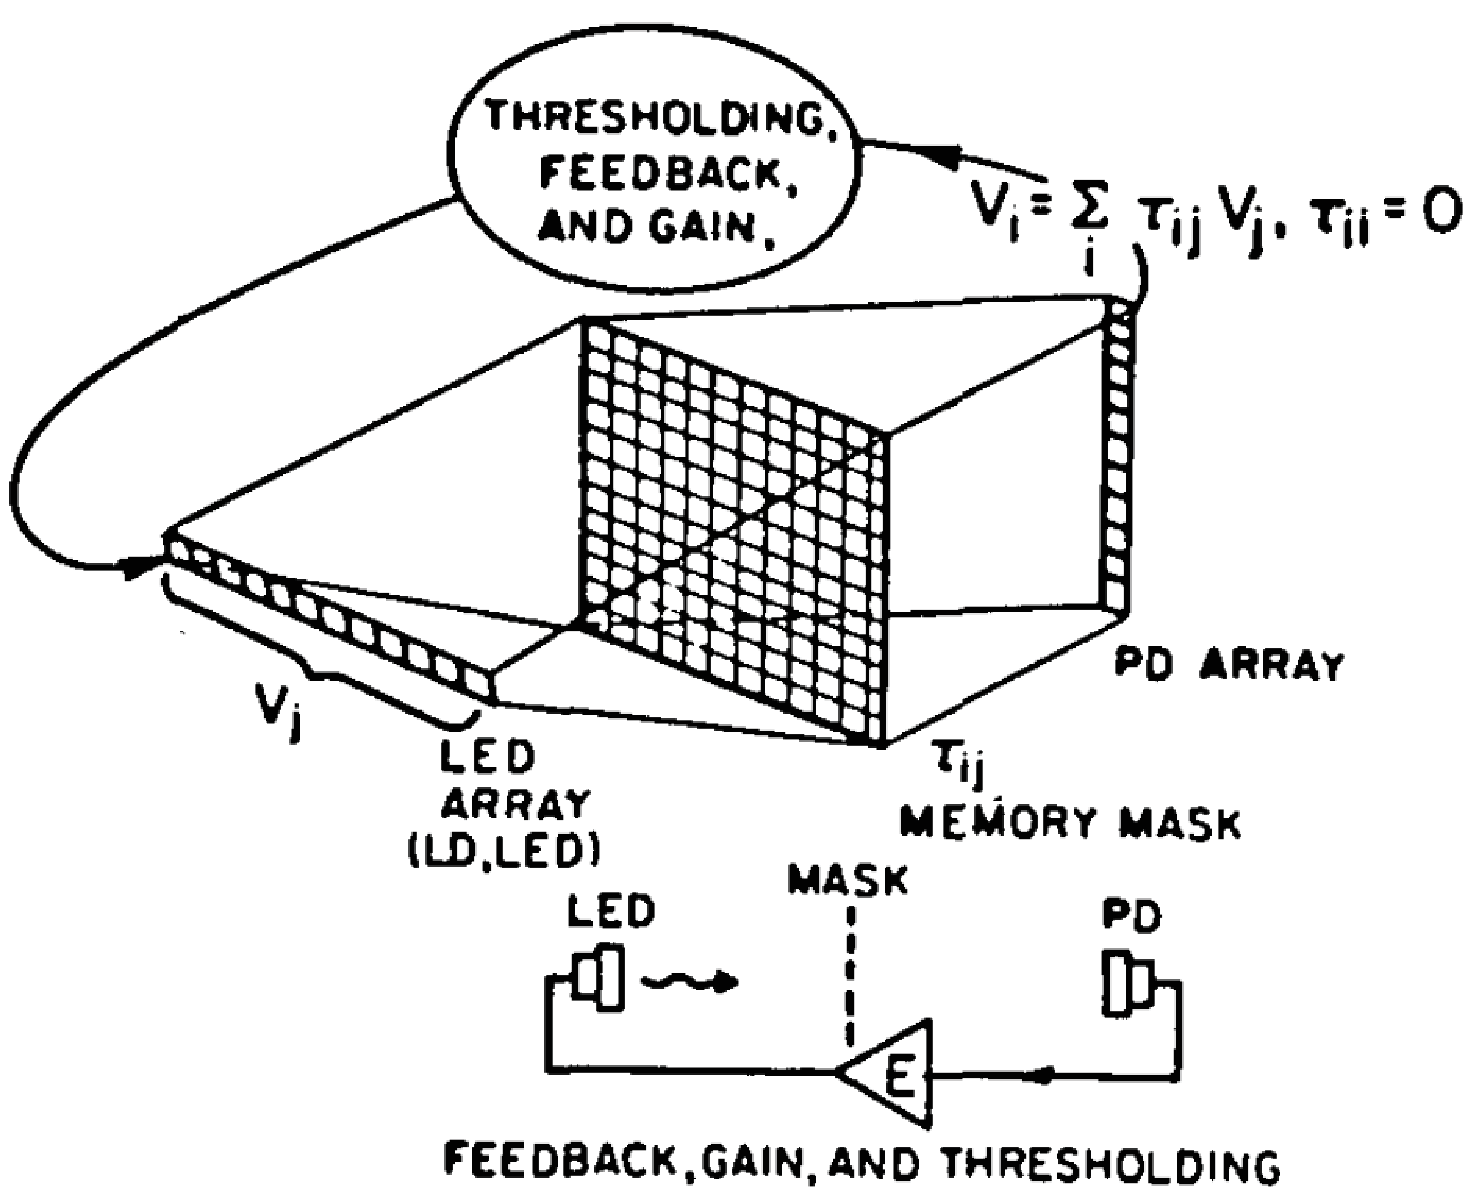
\includegraphics[width=8.6cm]{figures/_first_optical_neural_net.pdf}
\captionof{figure}{\label{fig:first_optical_neural_net}Schematic of the first optical neural network. From Ref.\,\onlinecite{faps1985}.\vspace{1em}}
The proposal for an optical neural network presented in Ref.\,\ref{psfa1985} was experimentally demonstrated by Farhat, Psaltis, Prata, and Paek, also in 1985 \cite{faps1985}. In that work, a Hopfield network was demonstrated, thus achieving an optical implementation of content-addressable associative memory. The experimental setup is shown in Fig.\,\ref{fig:first_optical_neural_net}. In this first construction of an optical Hopfield network demonstrated in Ref.\,\cite{faps1985}, LEDs played the role of the logic elements: the state of each neuron was represented by an LED (left of Fig.\,\ref{fig:first_optical_neural_net}(a)); with the LED off, the associated neuron state was equal to -1, while the LED being on represented the 1 state. The light from the LEDs then propagates through free space, interacts with a memory mask that implements matrix-vector multiplication, much like in the Stanford architecture \cite{godi1978}, and the outputs are detected on photodiodes. The system then implemented nonlinear iterative feedback to the matrix-vector multiplier. The nonlinear feedback was carried out by converting an optical signal to the electrical domain with the photodiode, applying gain and nonlinearity in the electronic domain, and converting back to optical with the current drive on each LED, although the intention was to eventually eliminate the intermediate electrical processing. In this construction, an array of LEDs represents the input vector, and an array of photodiodes detects the output vector. ``The output is thresholded and fed back in parallel to drive the corresponding elements of the LED array.'' Through the iterative procedure, the network reaches a steady state that corresponds to the retrieval of the intended memory. In this initial demonstration, a 32-neuron system was implemented with an array of 32 LEDs and 32 photodetectors. 

These original studies of optical neural networks sparked significant further interest in the subject. Multiple related research efforts branched off of this starting point. In 1986, Anderson implemented a different form of associative memory \cite{an1986} based on optical eigenstates in a resonator. As the author explained, ``A gain medium internal to the resonator amplifies the field belonging to the eigenmode that most resembles the injected field; the other eigenmodes are suppressed through a competition for the gain.'' In this concept, an optical resonator with spherical mirrors remembers Hermite Gaussian fields, and the stored information can be programmed by a user. Programming occurs by writing patterns in a volume hologram that plays the role of one of the mirrors. This original demonstration was able to recall one of two stored patterns based on input of part of one of the patterns.

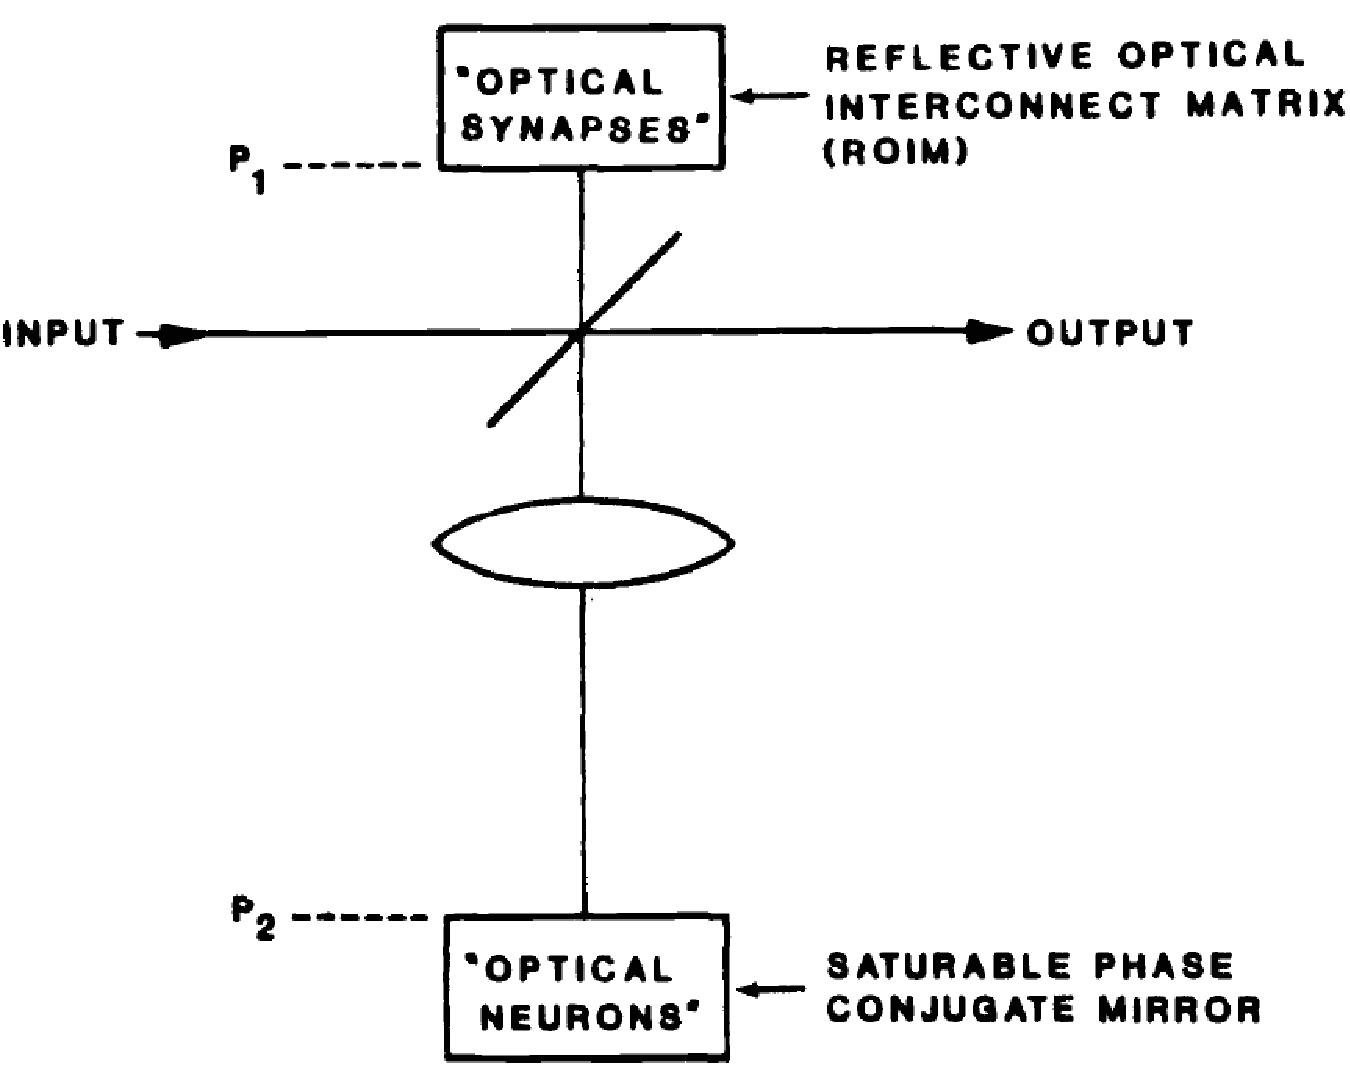
\includegraphics[width=8.6cm]{figures/_neuro_optic_processor.pdf}
\captionof{figure}{\label{fig:neuro_optic_processor}Schematic of the neuro-optic processor architecture. From Ref.\,\onlinecite{jast1986}.\vspace{1em}}
This idea of using a volume hologram to store memory took hold for optical neural network. In 1986, Jannson, Stoll, and Karaguleff studied the use of a volume hologram to store synaptic states, as shown in the schematic of Fig.\,\ref{fig:neuro_optic_processor}. While the optical apparatus is complex, requiring a saturable phase-conjugate mirror, the technique can lead to very high storage density. The idea is to have sources, such as the LEDs of Psaltis and Farhat, provide inputs, and use free-space propagation with optical components to steer the beams. The state of the neurons can be controlled by the intensity of the sources or by intensity modulation controlled by a spatial light modulator. But the interconnections between neurons\textemdash the synapses\textemdash are established and weighted based on the internal state of the volume hologram. Optical-wavelength-scale gratings written in the holographic medium route each input to many outputs, thereby utilizing the massive parallelism and connectivity of optics. In Ref.\,\cite{jast1986}, the authors calculate that this approach can realize $10^8$ neurons and $10^{16}$ synapses that can be trained on $10^6$ inputs. 

The use of volume holograms for storage of synaptic weights was further explored in subsequent years. In 1987, Wagner and Psaltis used holographic gratings in photorefractive crystals to store associative memories \cite{waps1987}. In a photorefractive crystal (often LiNbO$_3$), the memory is written through a procedure where input beams interfere with beams routed from target outputs to interfere within the crystal to establish the volume hologram by ionizing charge traps in the crystal and thereby modifying the index of refraction locally. As the authors stated, ``The recorded hologram is stored in the spatial distribution of the ionized traps in the crystal.'' Further, ``[W]e must...design a sequence of exposures that can load the appropriate weight values in the finite pool of trap sites that are available.'' The procedure implemented a Hebbian-type learning rule to achieve local (pairwise between neurons), associative learning. The networks had a multilayer, feed-forward architecture, and a form of backpropagation was used for training. The work introduced the use of a nonlinear etalon to achieve a sigmoidal response. The objective was still to achieve an associative memory, in this case for image classification. The concepts of this work bear strong resemblance to more modern deep learning, although the hardware is significantly different that what has become commonplace. The authors argued, ``This architecture combines the robustness of the distributed neural computation and the backpropagation learning procedure with the high speed processing of nonlinear etalons, the self-aligning ability of phase conjugate mirrors, and the massive storage capacity of volume holograms to produce a powerful and flexible optical processor.''

The photorefractive crystals that store the volume holograms in this architecture were investigated in more detail 1988 by Psaltis, Brady, and Wagner \cite{psbr1988}. The technique commonly employs phase-conjugate mirrors, which reflect light back along their original path. In Ref.\,\cite{psbr1988}, the objective was to derive fundamental limits to the number of interconnections that could be achieved in feed-forward neural networks using this approach to routing of free-space beams; the practical limits may be quite different. As the authors noted, ``...in an optical implementation each grating corresponds to a separate interconnection between two neurons....'' They further explain, ``There is a nice compatibility between simple (multiplicative) Hebbian learning and holography; the strength of the connection between two neurons can be modified by recording a hologram with light from the two neurons.'' The authors concluded, ``The density of interconnections which may be implemented in these crystals is limited by physical and geometrical constraints to the range of from $10^8$ to $10^{10}$ per cm$^3$. This extraordinary synaptic memory density, and the use of volume storage rather than surface storage, was a strong motivator for this work to persist. 
 
Other approaches for implementation of volume holograms were presented, including with liquid crystal gratings \cite{jaju1988}. In Ref.\,\cite{jaju1988}, it was also shown that two-state neurons (as utilized in a Hopfield network), could be implemented with liguid crystal optical switched. Beyond volume holograms, other approaches to photonic interconnection were championed. In 1987, Caulfield calculated that 2D arrays of inputs and outputs could be connected all-to-all using a spatial light modulator, in principle capable of achieving $10^{12}$ connections in a realistic system. In 1988, the group of Yariv utilized spatial light modulators located in a plane parallel to an array of detectors to achieve the synaptic connection matrix \cite{agne1988} in a Hopfield model with binary neurons. In 1989, a Hopfield neural network was implemented by Ito and Kitayama using optical fibers for interconnection between nodes. ``The coupling ratio from fiber to fiber represents the synaptic weight of the connection between units.'' In that work, a $5\times 5$ array was demonstrated, thus implementing $25^2$ connections. The light sources were compound-semiconductor laser diodes, and signals were detected with silicon photodetectors. In that approach, one network implemented nodes with positive weights, and another network implemented negative weights. In their 1989 review \cite{caki1989}, Caulfield, Kinser, and Rogers identify six optical interconnection methods present at that time: 1) fiber optic fan-in/fan-out; 2) holographic in-plane connection in integrated optics \cite{fees1988}; 3) optical parallel matrix-vector multipliers \cite{faps1985}; 4) lenslet-array multiple imaging \cite{fami1986}; 5) thick holographic associative networks; and 6) fixed hologram arrays \cite{ca1987}.

Spatial light modulators did not appear on the list, but have been considered for optical neural network applications. Farhat contributed a unique perspective in a 1987 article in which he sought to add artificial intelligence to conventional computer controllers through the hybrid integration of a learning optical system with a digital electronic control system. He focused on supervised learning by: ``1) computing the interconnectivity matrix for the associations that [are to be learned] and 2) changing the weights of the links between their neurons accordingly.'' ``Such self-organizing networks therefore have the ability to form and store their own internal representations of the associations that they are presented with.'' Specifically, Farhat intended to use optics to speed up the cumbersome learning/training phase of Boltzmann machines (see Sec.\,\ref{sec:overview_of_machine_learning}). He was using and LED array as the inputs to the network with a computer-controlled spatial light modulator to apply weights. Learning was achieved with an algorithm combining photodetection, electronic and computer processing, and feedack to update the SLM. Farhat explained his vision of the hybrid neural/digital system: ``[T]he addition of such a module to a computer-controller through a high-speed interface can be viewed as providing the computer-controller with artificial intelligence capabilities by imparting to it neural net attributes.''

In addition to the work discussed thus far, many other studies related to optical neural networks were conducted in the 1980s and 1990s \cite{fili1987,maar1987,safi1995,mo2000} before the field lost momentum for a duration. In the late 1990s and 2000s, the field of optical neural networks faced two strong headwinds. Optical computing had not found a technological niche or commercial foothold, and was thus in a state of disrepute. Simultaneously, neural networks had again fallen out of favor. At this time digital computing sailed forth on the wind of Moore. Applications of neural network concepts to optical systems maintained very tight focus on specific applications. For example, in 2003 Kawata and Hirose proposed an optical neural network concept that utilized the wave nature of light as well as frequency multiplexing to achieve a system that could learn appropriate phase values for a specific optical communications applications. The goal was not to compete with silicon microelectronics for a broad class of systems, but rather to perform one optics-related function at a level that could not be matched by electronics.

%Coherent optical neural network that learns desirable phase values
%\cite{kahi2003}
%-coherent optical neural network that learns a desired output phase as a function of frequency
%-uses liquid crystal SLM
%-very application-specific, intended to be used in optical communications or adaptive coherent optical image processing
%-parameters of neuron (inputs, outputs, weights) given complex values corresponding to light-wave properties
%-it is not clear how to utilize these wave properties of light in complex neural systems, as they require precise control at every synapse. we often would rather not have to keep track of all these parameters with control %knobs, and unsupervised means of utilizing them are not obvious.
%-more likely to me that specialized modules may utilize color and phase, but central cognitive module will be much simpler to ensure scalability
%-learning with complex-valued Hebbian rule, updates achieved with a computer changing SLM settings

%optical implementation of associative networks
%\cite{fili1987}
%-comparison of several optical associative networks
%-emphasis on multimodule approach, actually referring to network layers
%-layers are nonlinearly connected
%-each module (layer) is a complete, adaptive associative memory which can be modified by exposure to sets of associated information patterns, eg feature vectors
%-presentation of one pattern u should result in recall of paired pattern v
%-focused on optical hardware implementations for associative modules
%-argues that optics is better for low-precision analog arithmetic, but soens uses optics for binary communication, with analog operations performed in superconducting domain based on high beta L loops.
%-interesting summary of arguments in favor of optics for various computational tasks
%-proposals for optical holographic memories and optical perceptron neural networks go back to the 1960s (cite fili1987 and references therein)
%-dont need to discuss this paper in detail, just a review circa 1987 of optical approaches to associative memories, basically a published study by the navy

%Optical associative memory model based on neural networks having variable interconnection weights
%\cite{maar1987}
%-Modification to Hopfield network
%-Simulated results
%-No physical optical system built
%-Optics for readout in vector-matrix multiplication

%Optical learning neurochip with internal analog memory
A snapshot of the field in 1993 is captured in the Applied Optics feature issue edited by Wagner and Psaltis \cite{waps1993}. Here we highlight just one article from that issue. In the work by Nitta et al \cite{nioh1993} ...

%Adaptive multilayer optical neural network with optical thresholding
\cite{safi1995}

As the excitement around deep learning has grown in recent years, free-space optical neural networks have seen a resurgence. At least four new papers in this domain were published in 2018 \cite{buma2018,hasl2018,liri2018,chsi2018}. In Ref.\,\cite{buma2018} Bueno et al. pursued free-space optics for reservoir computing. They demonstrated an optical neural network based on a recurrent graph achieved with a spatial light modulator combined with a digital micro-mirror device accomplishing the variable weights of the output layer. The authors constructed a recurrent neural network of 900 nodes to serve as the reservoir (see Sec.\,\ref{sec:overview_of_machine_learning}). All connections established with the spatial light modulator were fixed and positive, while all training occurred in the output layer through the digital micro-mirror device that established binary weights. During training, the optoelectronic system steps through discrete time with a specified update equation. In this demonstration, update of 900 nodes occurred at 5\,Hz, limited by software control interface. The authors estimate the system could scale to $10^5$ interconnected nodes, which is a useful scale for reservoir computing. 

Another recent paper, this one by Hamerly et al., proposed a system leveraging many of the same free-space optical neural network concepts as have been discussed above with the new idea that the synaptic weights in a feed-forward neural network can be established through homodyne interference \cite{hasl2018}. In this case, synaptic weights are not established by diffractive optics, volume holograms, or spatial-light modulators, but rather by a complex configuration of modulators acting on a separate set of optical beam that interfere with the signals represent neuron activations. The signals from the output neurons are envisioned to be read out in a serial manner, thereby implementing a form of time-multiplexed readout to simplify hardware at the expense of operating speed. Nonlinearity is applied electronically, so the sole function of the complex optical apparatus is to perform matrix-vector multiplication\textemdash the exact same objective as the Stanford architecture of 1978. 

While the multi-homodyne approach adds optical complexity to the setup, an approach from the other end of the complexity spectrum has recently been demonstrated. The work by Lin et al. showed the use of terahertz sources in conjunction with diffractive gratings that were 3D-printed \cite{liri2018}. Multiple planes of diffractive elements were cascaded to arrive at the desired input-output transformation. In this case, all training and design of the feed-forward networks is carried out on external computers to arrive at a series of gratings achieving the desired network output, and the final gratings were simply printed (made possible by the large wavelength of terahertz light) and placed like cards in slots in the optical path. Using this approach, the team demonstrated MNIST and fashion MNIST classification (see Sec.\,\ref{sec:overview_of_machine_learning}).

The final recent paper on neural networks utilizing free-space optics to be discussed here illustrates the growing role of convolutional architectures for deep learning (see Sec.\,\ref{sec:overview_of_machine_learning}). In Ref.\,\ref{chsi2018}, Chang et al. explore the use of a free-space optical convolutional layer prior to electronic processing. The authors ``incorporate a layer of optical computing prior to either analog or digital electronic computing, improving performance while adding minimal electronic computational cost and processing time.'' They assume light is incoherent and monochromatic and make use of a phase mask in the Fourier plane to apply the optical transformation that implements the convolutional function. The objective is to utilize optics in the steps for which it is well-suited before transitioning to electronics for further processing, including nonlinearities. Such an approach is most likely to be advantageous if the input signal is already optical, most prominently in the context of imaging. As the authors state, ``[A]n imaging scenario where the input signal is already an optical signal easily allows for propagation through additional passive optical elements prior to sensor readout.'' Because such an approach results in more hardware complexity, as the neural network would require a free-space optical setup in addition to any electronics, it is most likely to be useful in artificial vision systems where free-space light is the signal, not when digital images need to be processed. In such cases, the efficiency of incorporating an optical convolutional layer optimized for a specific classification problem may save time and power.

%Large-scale optical neural networks based on photoelectric multiplication
%\cite{hasl2018}
%-extraordinary claim that an optical neural network can accomplish a multiply-accumulate operation with less than one photon of energy. they arrive at this number by assuming unity efficiency of photon generation, detection, no loss anywhere in the system, and some MACs can fail to occur without loss of classification accuracy due to the redundancy of the network
%-they argue the approach is scalable to $10^6$ neurons

In their 1990 review, ``Holography in Artificial Neural Networks'', Psaltis et al. summarized their work on optical neural networks \cite{psbr1990}. The authors list three primary motivations to move toward neural architectures: 1) massive parallelism; 2) dense interconnections; and 3) realizing computational systems that can learn. Decades later, the motivations are still the same, but the implementations have shifted from associative memories based on Hopfield-type networks to deep learning based on feed-forward neural networks. To our knowledge, no efforts based around the employment of free-space optical apparatus are focused on the construction of a system with general artificial intelligence. Nevertheless, while recent and ongoing work aspires to utilize free-space optics primarily for deep learning and reservoir computing, it is our goal to understand how these technologies may apply to the pursuit of systems capable of cognition. Toward this end, we must ask ourselves why these systems, with decades to incubate, have not displaced conventional hardware for neural networks and deep learning. To begin, Ref.\,\cite{agne1988} stated in 1988: ``Further advances in this field are...limited due to the absence of efficient and reliable hardware realizations of [neural network] models.'' While this may have been true, it ended up being the case that hardware advances in silicon microelectronics proved sufficiently efficient to initiate the presently occurring deep learning boom, thereby significantly reducing the motivation to develop new hardware, particularly drastically different hardware, such as free-space optics. 

However, the current deep learning boom is leading to rapid saturation of what CMOS hardware can achieve in this context. Moore and Dennard scaling will not provide the same fuel in the next thirty years as they did for the past thirty years, so is there a new reason to expect some of these concepts of free-space optics to have another chance at large-scale impact on neural networks in the modern context of deep learning? There are reasons to remain skeptical. Specifically regarding holographic connections written within the volume of a photorefractive crystal, the strength of each synapse is determined by optical amplitude during writing. A complex procedure of many exposures establishes synaptic weights, and writing each new synaptic weight can inadvertently modify others. Psaltis et al. wrote in 1990 ``Distributed connections have advantages and disadvantages\textemdash the disadvantage compared to the localized implementation is the reduced control of individual synapses. The adjustment of the strength of one synapse may inadvertently affect other synapses as well. Accommodating this limitation is perhaps the most crucial research issue in this field....'' This problem has not been solved. The density of this storage technique is extremely enticing, but so is the prospect of storing bits in electronic spins of single dopants densely embedded in a solid-state matrix. Accessing the information stored in the matrix is, however, extremely difficult. While extraordinary in principle, such technologies may be inaccessible in practice. While photorefractive media written into a hologram through the use of phase-conjugate mirrors is a beautiful use of sophisticated nonlinear optics, it not likely to be sufficiently advantageous to merit the incorporation of sensitive optical apparatus in mainstream computing technology.

More generally, as stated by Jutamulia and Yu \cite{juyu1996}, ``Neural networks that involve optical implementation are commonly called optical neural networks, although they should be correctly called hybrid optical neural networks....[T]hey always require non-linear functions that are difficult to implement optically. Most proposed optical neural networks leave this non-linear function to be implemented electronically.'' Nearly all efforts in optical neural nets are really efforts in optoelectronic neural nets, as the difficulties of working with bistable optical devices \cite{ke1985} have steered nearly all work to utilize optical-to-electrical conversion and electronic nonlinearities, with notable exceptions \cite{prsh2017,more_refs_here}. Thus, optoelectronic apparatus implementing neural systems must have electronic components as well as optical components, including passives as well as sources and detectors. For scalability under economic constraints, such hardware capable of outperforming silicon microelectronic circuits must integrate these components monolithically, or at least with a co-packaged, chiplet approach. The necessary levels of optoelectronic integration may just now be emerging as viable for the described task, driven by the digital computing applications of silicon photonics discussed in Sec.\,\ref{sec:integrated_silicon_photonics}. However, if such silicon photonics approaches are going to be employed, they will little resemble the hardware of free-space neural nets, as discussed below in Sec.\,\ref{sec:integrated_photonics_for_deep_learning}. There is one general class of reasons to expect that no free-space optical approach will gain widespread traction: free space optical components and systems are bulky and difficult to package, making fieldability expensive. The bulk nature makes it is difficult to engineer entire systems that are simply ``plug-and-play'' and do not require experience with optics to operate. Thus, scaling to large systems is problematic, as planar, many-step lithography cannot be used to construct many of the complex elements.

Specifically related to the subject of this article, new considerations arise when we consider hardware not for deep learning, but for active cognition. In this context, highly complex, recurrent and adaptive networks are required, as discussed in Sec.\,\ref{sec:neural_systems}. In terms of achieving the desired graph structures, free-space routing only moves light in straight lines, and it is difficult to construct modular and heirarchical recurrent graphs with interconnectivity required for cognition. For free-space optics, everything is most straightforwardly laid out in a series of planes, with light propagating between adjacent planes. Using light in this manner has the advantage that ``multiple beams of light can pass through lenses or prisms and still remain separate,'' \cite{abps1987} yet routing of free-space optical signals brings new challenges for complex neural systems. To achieve connectivity graphs corresponding to neural networks with feed-forward, feed-back, and recurrent connections, light cannot travel only in straight lines, but rather must branch and change direction many times, often being routed around obstacles formed by other parts of the network. Construction of complex networks with free-space optics, mirrors, and lenses quickly leads to issues related to scaling. Integrated photonic devices are likely much better suited to form the lateral and recurrent connections that are dominant in many regions of the brain. We will discuss in Sec.\,\ref{sec:soens} an architecture that combines integrated-photonic lateral connections with free-space feed-forward and feed-back communication as well as communication over optical fibers for long-haul signaling. 

Importantly, of this extensive body of literature regarding free-space optical neural networks, none relate to spiking neurons. As we have emphasized, the temporal dynamics and information processing in spiking neural networks is central to the mechanisms that underlie cognition. Similarly, all the approaches to optoelectronic neural systems discussed thus far implement only passive synapses and dendrites. Cognitive hardware requires much more complex functionality, including short- and long-term plasticity mechanisms as well as dendritic processing that are central to the manner in which spiking neurons adapt in time. These functions are best achieved with electronic components. The pursuit of sophisticated optical neural systems therefore intertwines with the exploration of neuromorphic electronics that is a stronger candidate for implementing computational functions, learning, and memory. Learning in free-space optical setups is not straightforward and almost always requires a supervised training algorithm with external computer/user control. Implementing learning through local plasticity operations, as is required for large-scale cognitive systems, is more tractable with electronic circuits. 

Finally, to my knowledge, all optical neural systems except the one our group has proposed encode synaptic weights in optical amplitude or intensity. In this way, some portion of the computation occurs in the optical domain. As we will argue in Sec.\,\ref{sec:soens}, this optical weighting results in energy and noise penalties. Instead, I will argue next that the proper role of light in neural systems is for communication only, and monolithic optoelectronic integration is required for complexity. Optical communication is likely to be carried out over integrated-photonic waveguides at the local scale, with free-space connections when suitable, and long-range communication over fiber optics. Before transitioning to a description of superconducting optoelectronic networks, let us first consider other contemporary approaches to machine learning with integrated photonics.

%-------------------------------
%misc notes on this section
%------------------------------
%-re: faps1985 LEDs were envisioned to be replaced by bistable optical devices (cite Keyes and his refutations)
%-holographic storage with free-space optics impractical to implement compared to integrated systems on a chip
%-emphasize strengths of optics: parallel processing and massive interconnection capabilities
%-downfall: the free-space optical setup is not conducive to fieldability or programmability. a software engineer cannot sit down at a computer and try new things. one needs a phd in optics to have any fun.
%-with soens, we must agree: such hardware will not be adopted instead of silicon microelectronics if the goal is moderate-scale Hopfield networks or similar machine learning systems. to displace CMOS, any new hardware must do something CMOS cannot do.
%-Need to mention here that the first optical neural networks by Psaltis intended to utilize incoherent LEDs because they are simple, scalable, and do not require precise control of phase across many optical paths.
%- in juyu1996, LEDs still prominent as sources \cite{juyu1996}
%-------------------------------
%end misc notes on this section
%------------------------------

\subsubsection{Machine learning with integrated photonics}
We have reviewed the history of optical logic devices, the rise of silicon photonics, and we have discussed many approaches to utilizing free-space optics for neural networks. We now consider more recent work that lies at the interface between integrated photonics, silicon photonics, and machine learning. 

As we have emphasized, in many artificial neural networks, the behavior of a neuron is modeled by Eq.\,\ref{eq:}. The linear portions of this operation reduce to matrix-vector multiplication. As noted above, matrix-vector multiplication has been a draw toward optics for some time \cite{godi1978,ve1984,maar1987}, with the Stanford architecture appearing on page one of volume two of Optics Letters \cite{godi1978}. Other approaches to matrix-vector multiplication have emerged over the years as technology has evolved, and one approach that is currently receiving attention is based on the concept introduced by Reck et al. in 1994 wherein a unitary matrix is implemented with an array of Mach-Zehnder interferometers \cite{reze1994}. With the addition of loss or gain, any matrix can be represented through its singular-value decomposition \cite{st2016}. Because additional MZIs can be used to discard light, the full singular-value decomposition and matrix-vector multiplication can be performed using MZIs. Implementation of such MZI networks with silicon photonic waveguides is currently being pursued \cite{mi2015,shha2017}, and it has been argued that efficient training through backpropagation can be implemented in optoelectronic integrated circuits with tunable MZIs and photodetectors working on conjunction with CMOS logic at each interferometer \cite{humi2018}.

In 2017, Shen et al. demonstrate the use of a network of Mach-Zehnder interferometers for classifying spoken digits \cite{shha2017}. The network was configured to accomplish the task through the use of thermooptic phase shifters perturbing the index of silicon waveguides. A network with four inputs and outputs was trained to classify four vowel sounds. The thermooptic phase shifters used in this system required 10\,mW per phase, and the number of phase settings required for a single-layer, feed-forward system scales as $N^2/2$ \cite{reze1994}. This power consumption is far too high to be competitive with other technologies for deep learning. However, other means of acquiring index perturbations may prove useful, such as non-volatile phase-change materials or microelectromechanical systems. In 2019, Fang et al. explored the implementation of a similar matrix-vector multiplier based on Mach-Zehnder interferometers wherein the phases were fixed at the time of fabrication based on optimization implemented in simulation. Such an approach is similar to the work of Ref.\,\cite{liri2018} discussed above wherein diffraction gratings were designed in simulated and then 3D-printed. This approach has the advantage of dissipating no power to maintain the phases, but the disadvantage that a system is purely static and is also susceptible to fabrication-induced errors that cannot be compensated during operation. 

If one wishes to employ feed-forward neural networks based on Mach-Zehnder matrix-vector multiplication that can be dynamically reconfigured to adapt to changing inputs, a suitable training procedure must be devised. Such a procedure, based on backpropagation was introduced by Hughes et al. in the group of Fan in 2018. The technique utilizes photodetectors and reconfigurable phase shifters controlled by transistor logic circuits at each Mach-Zehnder. During training, the algorithm requires light to first propogate forward through the network followed by light propagation in the opposite direction. The results from these two passes are stored in the logic circuits at each interferometer, an error signal is calculated, and the phase settings are adjusted. Such a system has not been demonstrated, but may be possible with ongoing advances in monolithic optoelectronic integration. The concept is reminiscent of the approach to backpropagation explored by Wagner and Psaltis in 1987 \cite{waps1987}. In other work from Fan's group, Williamson et al showed in simulations that such hardware can achieve a variety of nonlinear activation functions \cite{wihu2019}. The experimental results so far \cite{shha2017} have made use of nonlinearities applied in software, and other approaches to nonliearities have been proposed, usually based on optical nonlinearities such as in saturable absorbers that require high power and are difficult to fabricate at scale in the context of silicon photonics. The simulations of \cite{wihu2019} indicate that the required neuronal nonlinearities may be implemented through photodetection and and electronic reconfiguration of phase settings in interferometric devices. Hybrid devices utilizing a nonlinearity implemented with an electro-optic effect and electrical feedback have been studied since the early 1980s \cite{sm1980,ko1981}, but in early work primary attention was given to compound semiconductors, while silicon photonic implementations in conjunction with CMOS electronics are presently at the forefront. As the authors of Ref.\,\cite{wihu2019} state, the nonlinearity is achieved by ``converting a small portion of the original optical signal into an electrical voltage. The remaining portion of the original signal is phase modulated by this voltage as the signal passes through an interferometer. For an input signal with amplitude $z$, the resulting nonlinear optical activation, $f(z)$, is a result of the responses of the interferometer under modulation as well as the components in the electrical signal pathway.'' The nonlinearity is applied to an optical signal, but it is accomplished with electrical circuits, keeping with the assertions of Ref.\,\cite{juyu1996} that nonlinearities are best applied electronically, and only made conceivable in practice through decades of progress in silicon photonic optoelectronic integration. The nonlinearity is intended to be applied independently at each node of the neural network. Each node utilizes optical-to-electrical conversion with a waveguide-integrated photodetector, which converts optical current to electrical current, and a transimpedance amplifying stage, which converts electrical current to voltage. This voltage ``then passes through a nonlinear signal conditioner with a transfer function $H(\cdot)$.'' \cite{wihu2019} Implementing nonlinearity in this way leverages the strengths of electronics as well as optics. However, one motivation for optical matrix-vector multiplication\textemdash the light-speed-limited latency\textemdash is somewhat compromised. In this scheme, the electronic circuits need time to respond to detection and accomplish phase reconfiguration when new inputs are present. Reference \onlinecite{wihu2019} proposes to pass the optical signal to be modified through a delay line during this time. The electronic circuits can be quite fast, but nevertheless, this is an important conceptual consequence of the utilization of optoelectronic integration. 

In contemplating the recent work from Fan's group \cite{humi2018,wihu2019}, it is important to distinguish between interferometers comprising the matrix-vector multiplier and interferometers achieving the nonlinearities at present only at the nodes of each network layer. For the training scheme envisioned in Ref.\,\cite{humi2018}, photodetection and electrical reconfiguration of phase is required at each interferometer of the matrix-vector multiplier, of which there are $\mathcal{O}(N^2)$. These phase shifters dominate power and space consumption, as discussed in the next paragraph. By contrast, for the implementation of nonlinear activation functions envisioned in Ref.\,\cite{wihu2019}, only the output nodes of each network layer are involved, of which there are $\mathcal{O}(N)$. More power and space can be dedicated to these components because the scale as the number of neurons, not the number of synapses. The ideas presented in Refs.\,\onlinecite{humi2018} and \onlinecite{wihu2019} are some of the most compelling related to the use of contemporary optoelectronic integration capabilities to serve the functions of deep learning. Still, several features remain problematic: interferometers are used for routing between network nodes, so significant space is consumed; a number of phases proportional to the number of synapses must be controlled to establish the synaptic weights; and the use of a mesh of interferometers likely requires confinement of the routing infrastructure to a single plane. These challenges make lead to significant consumption of power and space and make it unclear whether such a technology will prove superior to silicon microelectronic approaches to deep learning, as we will now discuss.

Like its free-space counterparts before, matrix-vector multiplication with Mach-Zehnder meshes is intriguing for applications in feed-forward neural networks. However, there are reasons to be skeptical about whether it will outperform approaches based on customized silicon microelectronic circuits, such as tensor-processing units (see Sec.\,\ref{sec:semiconductor_neural_systems}).If power problems are addressed with static networks, an important part of what makes neural systems interesting\textemdash the ability to learn\textemdash is discarded. If adaptability is maintained, significant advances are required to achieve phase shifts with low power consumption and small footprint. A Mach-Zehnder is comprised of two directional couplers with a phase modulator between, and each of these components has non-negligible length when implimented in an integrated photonic setting. For a Mach-Zehnder mesh performing matrix-vector multiplication on an input vector of length $N$, the array will have the width of $N$ Mach-Zehnders and a length of at least $N/2$ Mach-Zehnders for the unitary part of the transformation alone. Loss regions necessary for a singular-value decomposition add further length. In a Mach-Zehnder interferometer, acquiring a phase shift through an electrooptic effect is characterized by a $V_{\pi}\cdot L$ product. Materials with non-vanishing linear electrooptic coefficient (Pockels effect) can achieve small $V_{\pi}$ with no current, and therefore no static power dissipation, but $L$ becomes quite large\textemdash on the order of centimeters. Employing the Pockels effect requires too much space for this application. On the other end of the spectrum, the thermooptic effect can reduce $L$ for a single Mach-Zehnder while maintaining modest $V_{pi}$ on the order of a few volts. However, this approach drives current through a resistive element to produce a temperature shift through Joule heating. $L$ can be reduced to the order of 100\,\textmu m (as was the case in Ref.\,\ref{shha2017}), but at the cost of significant power dissipation. Even with $L=$\,100\,\textmu m, the length of a chip becomes nearly 4\,cm for one feed-forward layer if $N = 784$, as would be the case for an introductory problem like MNIST. Additionally, use of the thermooptic effect leads to significant cross talk unless each device is spatially isolated, leading to further area consumption. Phase shifts induced by free carriers, such as proposed by Soref, fare no better, as they require modest $V_{\pi}$ and $L$ much greater than with the thermooptic effect. Even if phase shifts are static, written at the time of fabrication, Mach-Zehnders will occupy on the order of 100\,\textmu m, and therefore do not address the spatial scaling challenges of this approach to matrix-vector multiplication. This challenge has led the two senior authors of Ref.\,\cite{shha2017} to return to free-space approaches to matrix-vector multiplication for deep learning, stating ``the footprint of directional couplers and phase modulators makes scaling to large ($N\ge 1000)$ numbers of neurons very challenging.'' Nevertheless, the lead authors of Ref.\,\cite{shha2017} are pursuing this approach as a commercial product through start-up companies.

Spatial scaling is difficult for any integrated photonic technology due to the large wavelength of light relative to electrons. The reason why Mach-Zehnder meshes are even larger than other potential routing technologies is because all waveguides are laid out in a single plane. It is much more promising to use photonic interconnects between neurons if multiple planes of waveguides can be employed \cite{chbu2017,chbu2018,sami2017}, just like electrical interconnects would be unworkable if only a single plane of wires could be used. We will discuss multiplanar photonic interconnects in Sec.\,\ref{sec:comparison_of_interconnects}, but at present we conclude this discussion of matrix-vector multiplication with Mach-Zehnder meshes for deep learning by noting that spatial scaling is not the only formidable challenge of the approach. The fact that phase must be precisely controlled to establish the weight matrix. As Miller points out in considering optical logic devices, ``...coherent interference is mostly a nuisance in logic systems.'' \cite{mi2010} For training, this requires detection and phase control at every interferometer, and phase must be coherently re-established after each network layer. Loss from propagation through this long network is convoluted with the intended phase-induced amplitude modulation, and results in an error in signal that must be compensated. Further, because this is a non-spiking neural network, light sources are always on, and if the intention is to perform deep learning in data centers, compound semiconductor lasers operating at room temperature are likely to be employed. Thus, co-packaged light sources are required, most likely at each network layer. Reference \cite{wihu2019} has proposed nonlinear optical functions that do not require light sources at each network layer in principle, but in practice propagation losses through deep neural networks will become problematic if light levels are not restored. While this is an exciting opportunity for optoelectronic integration and technological exploration, it is not obvious such an approach will displace conventional silicon microelectronics for matrix-vector multiplication. The performance gains are likely to be modest at best, and if history is a guide, CMOS will not be displaced unless a competing technology can do something that CMOS simply cannot do.

Beyond considerations of power and spatial footprint, if we consider the application to cognitive systems rather than deep learning, the approach of using arrays of interferometers for routing and synaptic weighting is incompatible with large-scale cognitive systems for two primary reasons. First, as described in Sec.\,\ref{sec:neuroscience}, an important mechanism of learning in spiking neural systems is through STDP, wherein the activity of the two neurons associated with a synapse leads to memory adaptation. With interferometer arrays, changing a single phase in the network will, in general, modify many synaptic weights. This is similar to the limitation of writing synaptic weights as gratings in a holographic medium: the synapses are not independent. While backpropagation can be implemented with such a network \cite{humi2018}, STDP cannot. Second, this approach to routing is solely focused on achieving feed-forward graph structures and is not amenable to constructing recurrent neural networks with hieararchical modularity. Thus, matrix-vector multiplication via networks of interferometers is not likely to be the primary means of establishing synaptic weighting nor is it likely to achieve the complex structural graphs required of cognitive systems demonstrating general intelligence.


%An all-optical neuron with sigmoid activation function
\cite{mots2019}
-WDM input and weighting scheme
-logistic sigmoid activation function realized with a ``deeply-saturated differentially-biased Semiconductor Optical Amplifier-Mach-Zehnder Interferometer (SOA-MZI) followed by a SOA-Cross-Gain-Modulation (XGM) gate.''
-the goal seems to be a very close fit with a sigmoid, no matter the cost


Other efforts to utilize light for neuro-inspired machine learning are numerous. We now turn our attention away from feed-forward neural networks for deep learning and onto methods of using light for reservoir computing.

\subsubsection{Photonic Reservoir Computing}
We have summarized the concepts of reservoir computing in Sec.\,\ref{sec:overview_of_machine_learning}. Here we briefly summarize the state of the field of using light for reservoir computing. Reviews of the field of reservoir computing as a whole circa 2009 and 2019 can be found in Refs.\,\onlinecite{luja2009} and \onlinecite{taya2019}, respectively. Review regarding reservoir computing with photonic delay systems was published by Van der Sande, Brunner, Soriano in 2017 \cite{vabr2017}. There the authors state the primary motivation for reservoir computing: ``much of the promise of photonic reservoirs lies in their minimal hardware requirements, a tremendous advantage over other hardware-intensive neural network models.'' This advantage derives from the fact that connections within the reservoir are fixed, and only the output layer is trained. In the above discussion of using networks of Mach-Zehnder interferometers to accomplish the synaptic weight matrix we found that this network is very large in size due to the desire to control all synaptic weights. In that case, the network graph was feed forward, whereas in the case of reservoir computing, the reservoir is a recurrent graph with random, static connections. This changes the nature of considerations around connectivity between network nodes, generally easing the requirements on hardware. 

In photonic reservoir computing, there are two classes of approaches. In one class, the reservoir is comprised of multiple discrete optical nodes that each perform neuronal functions, whereas in the other class the reservoir is comprised of a single node, and the functions of different neurons are implemented serially in time. Elements of this latter class are referred to as \textit{delay systems}. We first discuss the former class and subsequently turn our attention to delay systems.

A significant body of work regarding reservoir computing systems that use light with spatially separate neuronal nodes has been put forth from Bienstman and co-workers. In the first papers on the subject, Vandoorne et al. proposed to use semiconductor optical amplifiers as the basic building blocks of the reservoir to explore pattern-recognition problems \cite{vadi2008,vada2011}. In this hardware implementation, the nonlinear dynamics results from interactions between photons and electrons in saturable semiconductor gain media. The motiviations to use this hardware implementation were fourfold: 1) semiconductor optical amplifiers have gain, so no separate component is needed to compensate for loss; 2) the devices are broadband, so fabrication tolerances are relaxed as compared to resonators; 3) their steady state characteristic resembles the upper part of a sigmoidal activation function, which is commonly used as a nonlinearity in neural networks, see Sec.\,\ref{sec:overview_of_machine_learning}), so knowledge gained from software may be applicable; and 4) such devices can be implemented in an integrated photonic circuit. Common materials for semiconductor optical amplifiers include compound semiconductors based on GaAs or InP. Reference \onlinecite{vadi2008} presented numerical simulations of a reservoir of 25 semiconductor optical amplifiers with limited connectivity motivated by the desire to avoid waveguide crossings within a single plane. It was found that this simple network was capable of accomplishing standard pattern recognition tasks. 

In systems making use of the carrier dynamics in semiconductor optical amplifiers or lasers, the memory time of integrating elements is set by the carrier lifetimes, which are in the range of 100\,ps-300\,ps. In Ref.\,\cite{vada2011}, Vandoorne et al. compared in simulation the performance of $9\times 9$ networks of semiconductor optical amplifiers to idealized nodes with a $tanh$ transfer function. That work investigated the sensitivity of the system to various design parameters and found that the system was most sensitive to the delays and phase shifts of the system's physical connections. Such a finding is intuitive considering propagation delays in a waveguide with group index of four are on the order of 100\,ps\textemdash the time constant of the memory elements\textemdash when propagating across a centimeter-scale chip. It is also reasonable to expect devices to be sensitive to phase errors when coherent signals are employed and input-output devices are phase-sensitive, as is the case with semiconductor optical amplifiers, reiterating Miller's observation that phase is more often a nuisance than attribute in large-scale optical information processing. Detection mechanisms that are insensitive to phase are more likely to be useful in very large cognitive systems. Noise from the semiconductor optical amplifiers was identified as problematic as well. Another interesting finding from this simulation comparing semiconductor optical amplifiers to $tanh$ nodes was that ``The result of the $\mathrm{tanh}$ network without leak rate at its optimal delay, is actually comparable to a tanh with leak rate and no (or minimal) delay. This reinforces the view that delay is an alternative approach to introducing memory next to leak rate.'' While this finding is limited in scope, it points to an important factor present in neural systems employing light for communication. Because the velocity of light is so much faster than axonal conduction, small-scale networks of artificial neurons employing optical communication do not generally utilize communication delay as a parameter to be utilized in information processing. Generally speaking, this is a tremendous strength of optical communication, and this finding by Vandoorne et al. indicates the potential for networks employing synaptic integration with a diversity of time constants to achieve similar functionality to systems using a diversity of delays. We will revisit this concept in Sec.\,\ref{sec:superconducting_optoelectronic}.

After the theoretical investigations just discussed \cite{vadi2008,vada2011}, Vandoorne, Bienstman, and co-workers turned their attention away from compound-semiconductor optical amplifiers as nodes of their reservoir and explored instead the use of free-carrier and thermal dynamics in silicon microrings to implement nonlinearities within a reservoir. In this concept, input optical signals are integrated within a microresonator with integration time set by the cavity $Q$, usually on the order of 100\,ps, like the relaxation time of free carrier in semiconductor optical amplifiers. As the intensity within the cavity grows, two-photon absorption increases, leading to a greater population of free carriers, which leads to further absorption as well as to heating as the free carriers relax and generate phonons. As the cavity heats, its index shifts due to the thermooptic effect, so the resonant frequency changes. The interaction between all these phenomena can lead to integration and bursting \cite{jobo2006}, forming a relaxation oscillator that may be likened to a spiking neuron. In theoretical analysis the authors considered free-carrier concentration and temperature as two dynamical variables to enable phase-plane analysis. These simulations guided the demonstration of cascadable excitation between two silicon microrings coupled through a waveguide. The combined dynamical effects of optical intensity, two-photon absorption, free-carrier absorption, heating, cooling, and thermooptic feedback make the system extremely difficult to model or control.

In subsequent work, Vandoorne, Bienstman and others utilized a silicon photonics chip in a purely linear, passive manner to pursue reservoir computing \cite{vame2014}. This work studied a $4\times 4$ mesh with each node connected to two other nodes in a swirl topology to avoid crossings. The connections were made through photonic delay stages achieving 280\,ps delay to reduce time scales to an experimentally accessible range. Each node could input and output light through grating couplers with off-chip sources coupled through optical fiber. Readout weights of the reservoir were implemented in software and were trained to implement Boolean logic functions with memory between bits at different temporal locations within a bit stream. For example, 2-bit XOR with one bit from the current time step and one bit from the previous time step was demonstrate. The various delay times incurred by different propagation pathways through the network made these delayed logical operations possible, and to perform XOR with bits with different delays, one must re-train the readout. Such a purely passive reservoir is not an end in itself, and in more recent theoretical work Denis-Le Coarer et al. combined the ideas of the free-carrier/thermooptic nonlinear resonator dynamics with the swirl-topology reservoir, again seeking to implement delayed XOR \cite{desc2018}. These simulations considered a $4\times 4$ grid of nodes with a ring resonator at each node. In simulation, the system can perform the delayed XOR task at 20 Gbps with error rates lower than $10^{-3}$ using 2.5\,mW of injected optical power. 

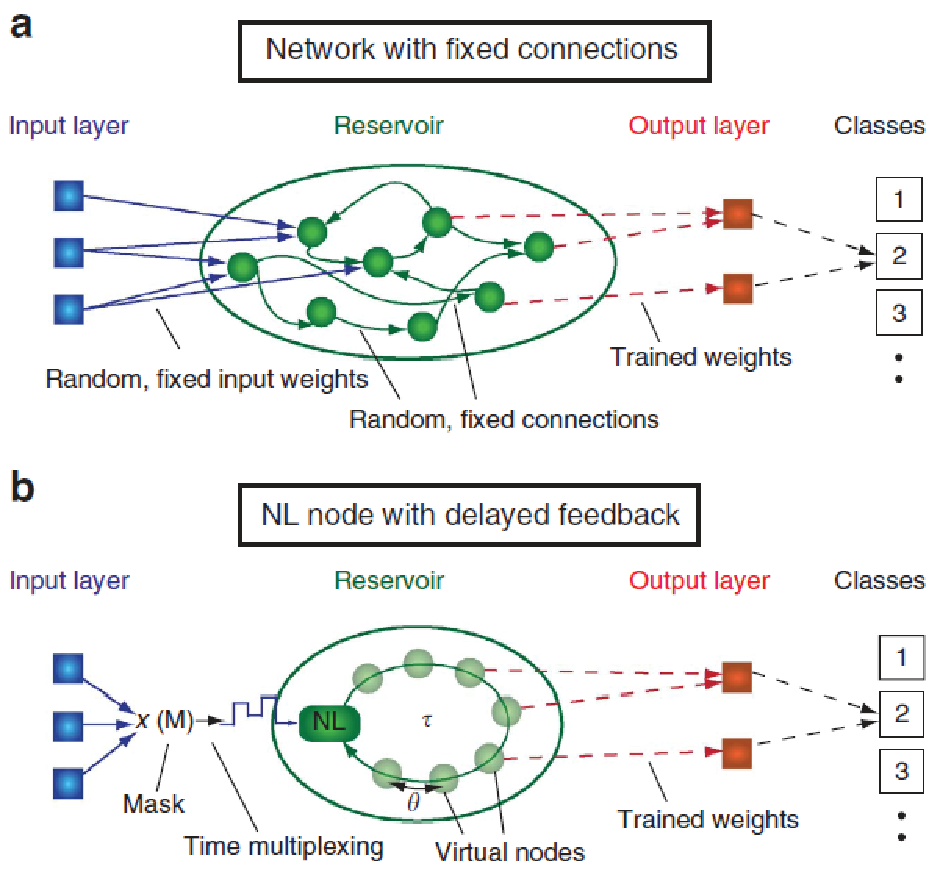
\includegraphics[width=8.6cm]{figures/_delay_systems.pdf}
\captionof{figure}{\label{fig:delay_systems}Schematic of the concept of reservoir computing with delay systems. From Ref.\,\onlinecite{apso2011}.\vspace{1em}}
In addition to these numerical and experimental studies related to using photonics for implementation of reservoir computing with arrays of discrete nodes, a significant body of work exists in the domain of using photonic systems to implement time-delay reservoir systems wherein each node is represented by activity at discrete times in a temporal train. In delay systems time is used to emulate space. This makes efficient use of hardware in that very few nodes can behave as many. We present a brief summary of the field here, and the 2018 tutorial article by Brunner et al. contains a comprehensive overview and bibliography \cite{brpe2018}. The delay concept is summarized in Fig.\,\ref{fig:delay_systems}, adapted from Ref.\,\cite{apso2011}. As stated in Ref.\,\cite{brpe2018}, ``Reservoir computers offer a compromise between performance and an implementation-friendly ANN topology.'' Specifically in the case of implementation of reservoir computers with delay systems, a signal circulates in a delay loop with total round-trip time $\tau$ (adopting notation from Ref.\,\cite{apso2011}). This total time is discretized into $N$ temporal intervals of fixed duration $\theta = \tau/N$. These temporal intervals are referred to as ``virtual nodes''. The signals input and output to and from the system during such an interval are inputs to and outputs from that virtual node associated with that time slot. The interactions between nodes depend on the temporal aspects of the various components of the circuit, and they are controlled by the temporal delay between two nodes, $\theta$. With $\theta$ very long relative to optical or electronic time constants, there is no interaction. With $\theta$ less than but on the order of these time constants, nearby nodes interact. The authors of Ref.\,\onlinecite{brpe2018} further explain, ``[S]implicity is bought in expense of time multiplexing and de-multiplexing in the input and readout layer.'' The expense can be quantified: ``[T]emporal multiplexing results in a reduction of the system's overall processing bandwidth by the number of neurons $N$.'' To increase the effective dimensionality of the system, the total delay time must be increased to allow inclusion of information from a larger number of virtual nodes. This reduces the speed with which a given computation can occur. It is also challenging to construct systems in which two distant nodes may interact without introducing interactions with all nodes in between. Such systems are useful in situations where power and hardware resources are at a premium.

Many results have been presented by the group of Fischer \cite{apso2011,laso2012,orso2015,brfi2015,brso2013,bubr2017,buma2018,brpe2018} as well as by the group of Massar \cite{padu2012,dusc2012,anha2017}. The first demonstration of this use of temporal delay in reservoir computing by Appeltant et al. occurred entirely in the electronic domain \cite{apso2011}. In that work, the authors defined delay systems as ``Nonlinear systems with delayed feedback and/or delayed coupling.'' Their delay system, implementing 400 nodes with a combination of bulk analog and digital electronics, was used to perform spoken digit recognition and as a model of a dynamical system in a benchmark task. In time-delay reservoir systems, training is most commonly conducted with standard techniques discussed in the review articles referenced above, employing supervisory control and postprocessing with an external computer. Backpropagation through time can also be used to train the readout layer, as discussed in Ref.\,\onlinecite{brpe2018}.

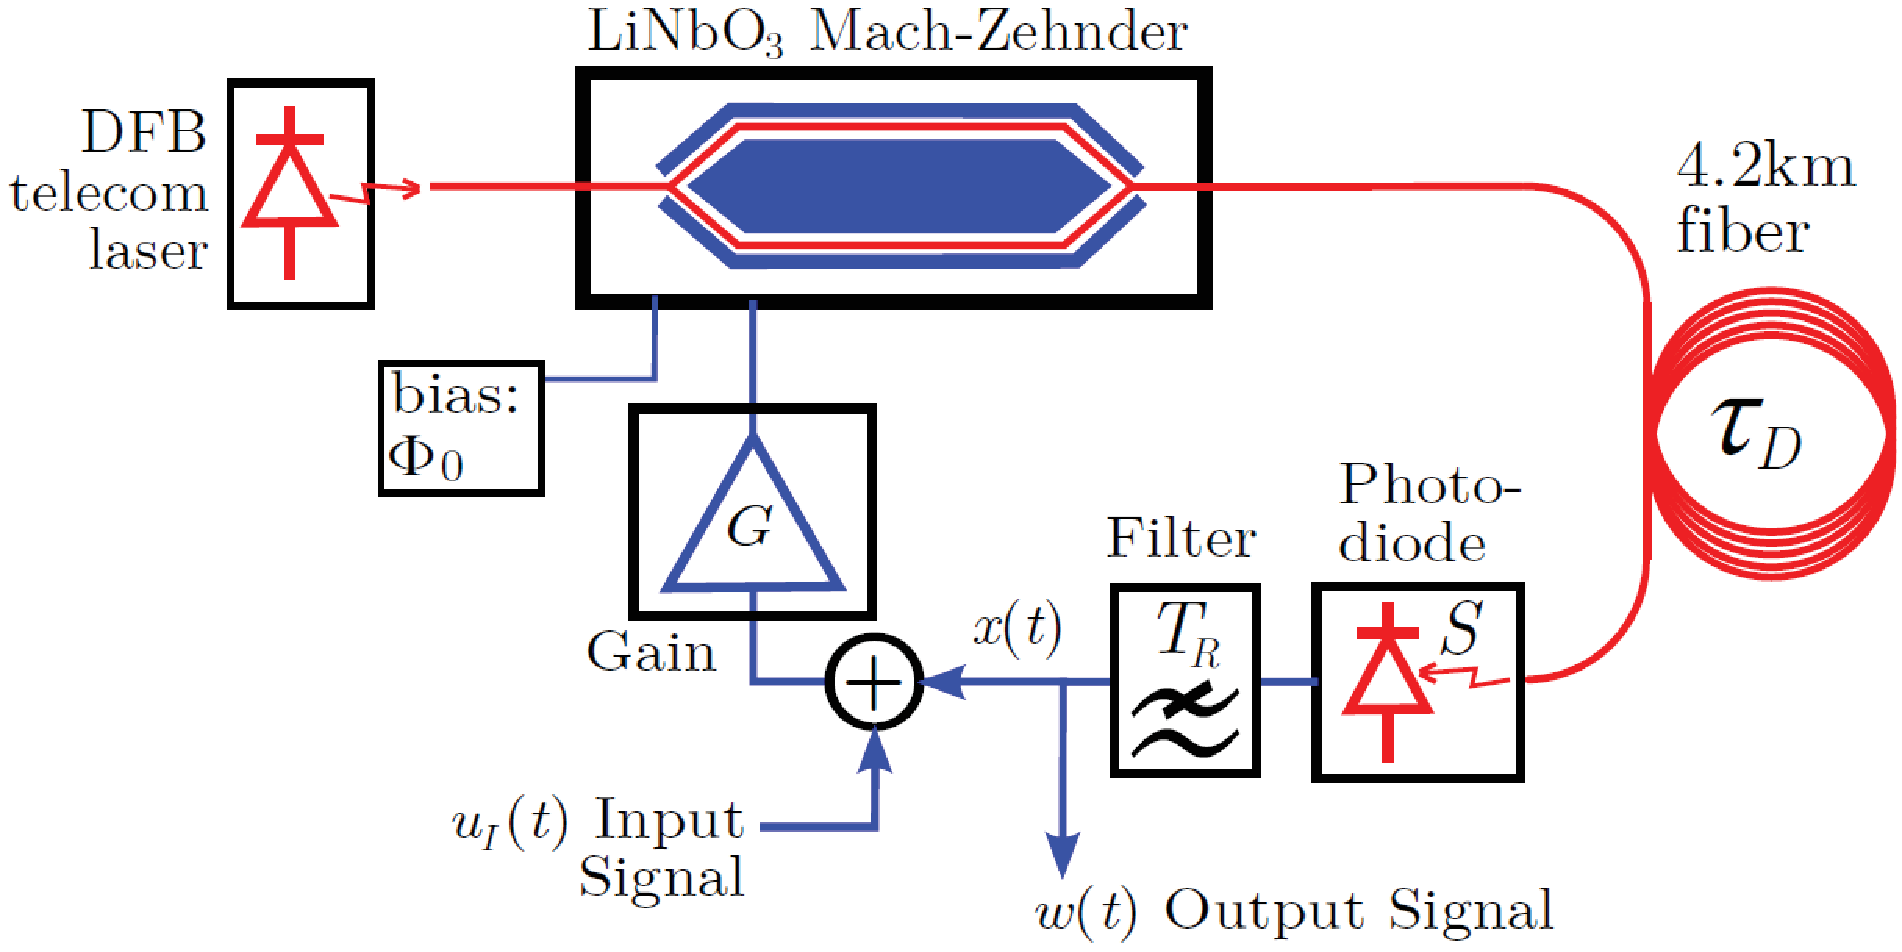
\includegraphics[width=8.6cm]{figures/_optoelectronic_delay_system.pdf}
\captionof{figure}{\label{fig:optoelectronic_delay_system}Hardware implementation of a photonic delay system for reservoir computing. From Ref.\,\onlinecite{laso2012}.\vspace{1em}}
Following on the work by Appeltant, two concurrent experiments from different groups demonstrated the use of light in a delay system for reservoir computing \cite{padu2012,laso2012}. References \onlinecite{padu2012} and \onlinecite{laso2012} employed similar concepts to the work of Ref.\,\onlinecite{apso2011} but the signal circulating through the delay system was now optical. The Architecture of the dynamical node is shown in Fig.\,\ref{fig:optoelectronic_delay_system} (use fig 2 of laso2012)(consider using Figs. 9,10 of \cite{vabr2017} to summarize delay systems). An input laser was modulated by a standard LiNbO$_3$ optical modulator to provide a nonlinear transfer function ($\mathrm{sin}^2$). The delay loop is based on an optical fiber spool. The optical signal is converted to the electrical domain on a photodiode. Within the electrical circuitry, multiple functions are performed. Low pass filtering occurs, information regarding inputs is added to the delayed signal, and amplification is introduced before the electrical output is used to drive the optical modulator, thus closing the optoelectronic feedback loop. Reference \onlinecite{laso2012} showed the use of the optoelectronic delay system to implement 400 virtual nodes accomplishing a spoken digit recognition task as well as a one-time-step prediction task leveraging fading memory. Reference \onlinecite{padu2012} implemented 50 nodes and also considered a spoken digit recognition as well as the simulation of a nonlinear auto regressive moving average equation and the equalization of a nonlinear channel. 

In subsequent work by Duport et al. in 2012, a similar photonic delay system was utilized, except the electronic feedback was replaced by a semiconductor optical amplifier, enabling use of the term ``all-optical'' reservoir computing \cite{dusc2012}. Similarly, work by Brunner et al. submitted in 2012 moved to utilization of a semiconductor laser cavity for nonlinearity rather than use electrical nonlinearities \cite{brso2013}. These approaches eliminate slower electronic circuitry, enabling high-speed information processing. For example, Ref.\,\onlinecite{brso2013} showed chaotic time-series prediction at a data rate beyond one gigabyte per second. Reference \onlinecite{bubr2017} explored the system with delayed optical feedback into a semiconductor laser in more detail, directly connecting ``physical properties of induced dynamical responses to the system's performance in a non-linear prediction task.'' This work explored operating conditions enabling high consistency of dynamical response to identical inputs while maintaining memory retention, identifying an operating point achieving a compromise between consistency and memory. 

Other work in this area identified the theoretical continuity from extreme learning machines to echo state networks and showed that both can be implemented with a single hardware platform, switching between the two by activating or deactivating a single physical connection \cite{orso2015}. Finally, as a concluding illustration of the potential and applications of reservoir computing based on photonic delay systems, the work of Antonik et al. in 2017 investigated the ability of such systems to achieve long-term prediction of time series by feeding the output from a reservoir back to itself. As the authors state, ``In previous experiments, the output was uncoupled from the system and, in most cases, simply computed off-line on a postprocessing computer. However, numerical investigations have shown that feeding the output back into the reservoir opens the possibility of long-horizon time-series forecasting.'' Application of this work are to understand the means by which biological circuits generate time series as well as to enable technological generation of time series with photonic reservoir computing. In this work, the readout utilized a field-programmable gate array. ``The use of hi-speed dedicated electronics makes it possible to compute the output signal in real time and feed it back into the reservoir.'' The general architecture was similar to that employed in Refs.\,\onlinecite{apso2011,padu2012,laso2012}. This work marks a new direction and potentially new application spaces for photonic delay systems.

Based on this brief summary of photonic delay systems for reservoir computing, can we gain insight toward our objective of designing hardware for general intelligence? In this case, the primary objective of reservoir computing is to simplify the network by reducing the number of degrees of freedom to be controlled by only training the readout layer. Further, in delay systems, the objective is to simplify hardware by utilizing only a single physical node to implement many virtual nodes. Nobody in this field is attempting to construct systems with general intelligence. Quite the opposite, the goal is to identify hardware that is simple to configure and capable of specific computational tasks. Still, it is useful to consider the specific reasons why time-delay systems are poorly matched to the functions underlying general intelligence discussed in Sec.\,\ref{sec:neural_systems}.

Time-delay systems are an approach to reservoir computing that minimize the demands on hardware by extending computation across time rather than across space. The state of a node during a time window in a delay system corresponds to the state of a node at a spatial location in a neural network. Such an approach is appealing in the context of emerging hardware because a system comprising only a single node can perform a useful calculation, albeit with a slowdown due to time multiplexing proportional to the number of emulated nodes. In Ref.\,\cite{brpe2018}, the authors emphasize that in a delay system, ``[A]ll nonlinear transformations carried out by the virtual spatiotemporal network rely on the same physical component.'' The is the primary limitation to achieving complexity in such systems. The single node of the system quickly becomes a bottleneck, as all spatial degrees of freedom are represented as temporal degrees of freedom. 

This delay technique is a form of time multiplexing, and as such scaling results in latency that scales with the number of virtual nodes. The time allocated to each virtual node is set by the characteristic time of relaxation oscillations in the physical system employed. For carrier dynamics in semiconductor optical devices, this is on the order of 200\,ps. One can simulate roughly 5,000 neurons in a microsecond, 5 million neurons in a millisecond, and the scale of cortex would require 10 seconds, meaning information from each node in the entire network cannot be accessed more frequently than this. Beyond the scale of a few thousand nodes, other hardware approaches are likely to have superior performance. This consideration summarizes the speed limitation resulting from time multiplexing on a single high-speed node, but one may argue that information exchange across a cognitive system within 10 seconds is not too bad. Due to limitations on the network architectures that can be achieved, simply sampling each virtual node during each delay cycle does not mean each virtual node has an opportunity to communicate with all other virtual nodes during each cycle. Network average path lengths, which in this case refer to the number of delay cycles that must take place for one node to communicate to another node, become very long. Long path lengths are not surprising in this context, considering the approach collapses all spatial degrees of freedom to a single temporal dimension. The nature of the interactions between virtual nodes in such systems is that only nodes close in time can interact with one another, and two distant nodes cannot have strong interactions without even stronger interactions with the nodes between. This assignment of space to time is not conducive to the fractal use of space and time associated with cognition. New concepts are required if small-world or modular, hierarchical networks are to be utilized. It is likely these new concepts will require more nodes with more complex spatial configuration.

\vspace{3em}
%All-{O}ptical {R}eservoir {C}omputing on a {P}hotonic {C}hip {U}sing {S}ilicon-{B}ased {R}ing {R}esonators
\cite{cosc2018} 

%Delay dynamics of neuromorphic optoelectronic nanoscale resonators: {P}erspectives and applications
\cite{rofi2017}

\subsubsection{Spiking Neurons with Semiconductor Lasers}
-separate by laser type, VCSELs, semiconductor ring lasers, fiber lasers
-note that these experiments are not included in the section on free-space implementations, but many of them use free-space optics
-the point of this section is specifically on the use of semiconductor lasers to produce pulses; if free-space optics are used, the same weaknesses apply

While the interferometric approach to deep learning discussed above makes use of static neurons, several approaches to spiking neurons have been pursued as well. One class of spiking photonic neurons leverages the carrier dynamics in compound semiconductor laser cavities. The equation governing lasers with gain and saturable absorber regions are isomorphic to the leaky integrate-and-fire neuron \cite{dukr1999}, with the number of excited carriers in the laser playing the role of the membrane potential. This correspondence has led to several designs \cite{nata2013} and experimental efforts (see Ref.\,\cite{prsh2017} and reference therein for a complete bibliography) to leverage this behavior to make spiking neurons that sum optical signals and produce optical pulses when a threshold has been reached. This work began in Er-doped fibers, and continues with on-chip implementations with III-V photonic systems, with much of the work being done in the group of Prucnal at Princeton. The refractory period of such neurons is set by the cavity photon decay time and is on the order of 10\,ps, while the integration time is set by the carrier relaxation time, and is on the order of 100\,ps. This short refractory period means such neurons can fire up to $10^9$ times faster than biological neurons, yet the short integration time means temporal correlations among neuronal firing events are forgotten rapidly, and the inability to broadly tune this time scale points to the potential for advantages to be gained from optoelectronic integration. 

While the goal of these efforts in excitable lasers is to perform neuro-inspired computing very rapidly with small networks, and not to achieve brain-scale systems, we nevertheless point out two features of this approach to using light in neural systems that are not conducive to achieving large-scale systems. The first is power consumption. To properly set the threshold of these neurons, the gain region must be continuously pumped. This requires between 100\,mW and 1\,W per neuron, even when the neuron is not firing. For a system of $10^{10}$ neurons, a gigawatt would be consumed, even with the system at rest. The second limitation regards computation. As discussed in Sec.\,\ref{sec:neuroscience}, neural information processing leverages many complex computations in synapses, dendrites, and neurons. In excitable lasers, all the computation occurs in the interaction between photons and carriers in the laser cavity. Multiply-accumulate operations can be performed with leak and threshold, but no path toward short-term synaptic plasticity or dendritic processing have been proposed. By relying on the exponential decay constants of photons and carriers, one is unable to tune the range of temporal information processing or supply the dendritic arbor with information across a wide range of temporal scales. These computations and time constants are more readily achieved in the electronic domain with circuits that can be engineered to perform complex functions rather than relying on material parameters, a point we revisit below.

%Neural network using longitudinal modes of an injection laser with external feedback
\cite{cosc1996}
-Colack et al.
-competition between modes in a laser cavity
-``A new optical neural-network concept using the control of the modes of an injection laser by external feedback is described by a simple laser model. This approach uses the wavelength dispersed longitudinal modes of the laser as neurons and the amount of external feedback as connection weights.''
-Simulations and experiments with GaAlAs injection lasers
-``The inputs and connection weights to this laser neural network are provided by external masks which control the amount of feedback reaching the laser.''
-stochastic learning employed
-Winner-take-all and XOR operations are performed, depending on the mask
-very high speed operation, measured in giga connections per second
-``In this report, we focus on utilizing the longitudinal modes and obtain the desired nonlinearities in the frequency domain in a single laser, rather than the spatial domain.''
-Summation and a sigmoidal activation function are modeled. In this case, the sigmoidal activation function provides a nonlinear response of the number of photons in mode $m$ as a function of the output power reflected back into cavity mode $m$.
-The sigmoidal saturation is due to competition with other modes and is controlled with external masks.
-This is in the steady state, not a model of spiking neurons

%Optical mode neural network by use of the nonlinear response of a laser diode to external optical feedback 
\cite{mosc1997}
-Mos et al.
-competition between modes in a laser cavity

%Optical neuron by use of a laser diode with injection seeding and external optical feedback
\cite{moho2000}
-Mos et al.
-All-optical neuron
-multimode laser diode
-inputs are applied and threshold is achieved in the optical domain, they cite Jutamulia \cite{juyu1996} regarding nonlinearity applied in electrical domain and consider optical thresholding one of the strengths of this work.
-The shape of the threshold function is adjusted through external feedback
-One of the two cavity modes corresponds to the output of the neuron, and when light is injected at this wavelength, it is an excitatory input
-The other cavity mode competes for gain, so light injected at this wavelength accomplishes inhibition
-Free-space optics are used
-Envision wavelength conversion to turn laser output to inhibitory signal
-Envision weighted interconnection between lasers using a free-space optical matrix vector multiplier and they cite Goodman 1978, Stanford architecture \cite{godi1978}
-Again, amplitude of optical signal is weight
-Also suggest a number of wavelength converters, pointing toward WDM inputs with the various wavelengths competing for gain: ``Due to mode competition only the wavelength with the highest amout of summed excitatory input will lase, suppressing laser action at any other wavelength.'' Similar work on winner-take-all competition in multimode laser cavities in \cite{cosc1996,mosc1997}

%Synchronization of laser oscillators, associative memory, and optical neurocomputing
\cite{hoiz2000}
-Hoppensteadt and Izhikevich
-Consider oscillatory neurons communicating via phases rather than amplitudes
-``Memorized patterns correspond to synchronized states where the neurons oscillate with equal frequencies and with prescribed phase relations.''
-``...motivated by the theoretical and experimental observations that cortical neurons are sensitive to the fine temporal structure (timing or phase) of the incoming pulse train.'' Such an idea would eventually lead to optical spiking neurons
-theoretical study
-assuming holographic interconnection medium


%Tunable vertical-cavity surface-emitting laser with feedback to implement a pulsed neural model. 1. {P}rinciples and experimental demonstration
\cite{rowa2007a}
-Romariz and Wagner
-companion paper to rowa2007b
-good introduction to motivations for spike coding
-``An optical approach with a potential impact on this field of research has to implement important dynamic aspects of these pulsing models in a simple setup, with the capacity for integration in large arrays. The pulsing optical neurons should easily combine optical and electrical input signals. The necessary nonlinearities should neither require high-power optics nor complex electronic circuitry. And it should be able to utilize the other key advantages of optical approaches including massive parallelism and global interconnection capabilities.''
-Neurons similar to FitzHugh-Nagumo model
-``The system employs the wavelength tunability of a semiconductor laser source, the nonlinear response (in wavelength) of a birefringence-based filter, and simple linear electronic feedback. Surprisingly, nonlinear dynamical behavior can be achieved with only linear optical and electronic components by using this mechanism of wavelength tunability.''
-consider using Fig. 1
-As opposed to utilizing nonlinear variation material properties with intensity, this work uses variation in laser wavelength. ``The fundamental idea behind this approach is that the intensity output of a spectrally selective linear optical system can vary nonlinearly with wavelength. If this modulated intensity is detected and the photocurrent is used to drive the electronic system that modulates the laser wavelength, complex nonlinear dynamics can result.''
-``The wavelength variable was previously explored in a static ANN implementation in the work by Mos et al. \cite{moju2000}. Specifically, the authors explore the fact that the amount of power emitted by a laser diode in a particular wavelength varies nonlinearly with the amount of optical power seeded to the cavity in the same wavelength. Our approach is different, though, in the use of external linear electronic feedback only, whose parameters are easier to control.''
-``The implementation described here is based on the concept of birefringent phase delay and its variation with wavelength.''
-``...establish a feedback loop by using the detected signal as the input to the circuit that produces the driving current $i(t)$.'' Make comparison to using detected signal to drive MZI in photonic delay systems
-Why don't we plan to make neurons this way? This approach with free-space optics and electrical feedback to bulk optical components is must less conducive to scaling that the approach with simple, pulsed, waveguide-integrated silicon LEDs and dense integration with basic superconducting electronic circuits. Our light levels are lower by orders of magnitude, and our approach does not hinge on the control and tuning of resonant frequencies of many coupled optical cavities or emission wavelengths of many coupled lasers
-use single-mode VCSEL, consider incorporating Fig. 5. Fig. 5 demonstrates why such an approach is difficult to scale. Goes back to the basic challenges of scaling free-space optical devices. 
-``In the regime explored here, the wavelength modulation mechanism is mainly thermal: current injection increases the temperature, and hence the index of refraction, as well as the cavity length through thermal expansion.''

%Tunable vertical-cavity surface-emitting laser with feedback to implement a pulsed neural model. 2. {H}igh-frequency effects and optical coupling
\cite{rowa2007b}
-Romariz and Wagner
-companion paper to rowa2007a
-LiNbO$_3$ is birefringent crystal
-VCSEL emisison demonstrates pulsing and bursting at 1.2\,MHz seen in simulation and experiments. However, output amplitude is not constant, indicating spikes are not binary communication events, and neuron output amplitude is convoluted with synaptic weights. The best way to deal with this is to utilize detectors that have an amplitude-independent response, and this precludes encoding synaptic weight in optical amplitude.
-This paper shows coupling between two such neurons, referred to as sending and receiving circuits. Challenges to mutual coupling of many such neurons are discussed. Some of these challenges can be understood from the following comments: ``When optical coupling is allowed, the receiving circuit spikes are more frequent (but irregular, and not in one-to-one relationship to the sending circuit). Individual oscillator conditions are too different here to allow locking with weak coupling. The receiving circuit produced oscillations more easily, probably because of a smaller threshold of its VCSEL. A few adjustments in the optical feedback circuit were done to have similar dynamic conditions for both circuits. After that, the receiving circuit was biased to instability, and when coupling was established the waveform of the receiving circuits became much more regular.'' These challenges point to problems with device variations, requirements for critical biasing, and related challenges that preclude scaling to billions of interconnected neurons, even before challenges with bulk optics are considered. Challenges with bulk optics are summarized in the comment by the author: ``In combining more than one VCSEL, the most difficult part was guaranteeing the uniform collimation and alignment of all beams.'' This challenge was encountered with coupling two such devices. Coupling billions with modular, hierarchical graphs structures is infeasible with free-space coupling using bulk optics.
-Pulsing in 1-5\,MHz range limited by thermal effects in VCSELs.

%Optical neuron using polarisation switching in a 1550nm-VCSEL
\cite{huhe2010}
-Hurtado et al.
-Uses two different polarizations, one for excitation and one for inhibition
-solve none of the problems of rowa2017a and rowa2017b

%A high performance photonic pulse processing device
\cite{rokr2009}
-Rosenbluth et al., Prucnal last author
-initial paper before krro2011 demonstrating some of the desired neuron functions

%Ultrafast all-optical implementation of a leaky integrate-and-fire neuron
\cite{krro2011}
-focused on enabling high speed, trying to simply go faster than VLSI approaches
-follow on to \cite{rokr2009}
-based on the metric of speed alone, the authors claim these neurons, ``significantly outperform VLSI circuit-based neurons,'' citing Ref.\,\onlinecite{voma2007}
-leaky integrate-and-fire model
-``The entire setup is based on fiber optic components operating in the 1550 nm telecommunication band.'' This work is an effort to employ concepts from fiber optic networks used in telecommunications for neural computing. While the hardware may be suited for the former application, it is not well suited to the latter.
-all-optical thresholders
-this approach has no potential for scaling due to fan in problems, power consumption, and general complexity of combining many components in fiber-optic apparatus, but the authors only seem to care about speed relative to CMOS neurons

%excitability in a semiconductor laser with saturable absorber
\cite{baku2011}
-three classes of excitability: class 1-the frequency of self-oscillations is zero at the transition (or bifurcation) point, class 2-oscillations are born with nonzero frequency, class 3-excitability is related to a specific transition to Q-switch-like pulsing through a homoclinic bifurcation in lasers with SA
-focus on class III excitability ``which arises as a competition between gain and saturable absorption in an incoherently pumped device.'' 
-class III is particularly useful because pulses are very fast and coherence is not required
-demonstration based on VCSEL (two InGaAs/AlGaAs quantum wells) grown with one more quantum well for a saturable absorber

%A leaky integrate-and-fire laser neuron for ultrafast cognitive computing
\cite{nash2013}
-Nahmias et al. (Shastri, Tait, Prucnal)
-Design of new laser
-leaky integrate-and-fire model
-based on VCSEL with integrated saturable absorber
-similar design to baku2011

%Solitary and coupled semiconductor ring lasers as optical spiking neurons
\cite{coge2011}
-Coomans et al
-theoretical
-semiconductor ring lasers
-behavior very sensitive to phase of driving pulses relative to phase of field within cavity
-two coupled rings simulated, phase and frequency sensitivity barriers to scaling

%Investigation of vertical cavity surface emitting laser dynamics for neuromorphic photonic systems
\cite{husc2012}
-in short, utilization of cavity dynamics in semiconductor lasers does not offer the controllable functionality to be a promising computational primitive in neural systems. Yes, these devices do exhibit neuron-like nonlinearities and pulsing behavior on very fast timescales, but this does not mean they are scalable neural computing leading to cognitive systems.
-they have high fan-out, but not high fan-in. for fan-in to a single mode device, all inputs must be coupled to that mode. 
-like their previous work (\cite{huhe2010}), they use polarization switching in VCSELs
-laser nonlinear dynamics result from carrier-photon coupling and lead to highly complex behaviors that are not easily controlled or tuned

%Excitability in optically injected microdisk lasers with phase controlled excitatory and inhibitory response
\cite{alva2013}
-Ghent/Bienstman
-make comparison to pulsing si microrings used for reservoir computing
-demonstrate class I excitability in optically injected microdisk lasers and propose a possible optical spiking neuron design
-threshold and integrating behavior
-optical phase control can be used to generate inhibitory response
-input pulse power around 1uW for 0.2 ns for threshold
-no transfer of excitation between disks demonstrated

%Relative refractory period in an excitable semiconductor laser
\cite{sebr2014}
-Selmi et al.
-``neuronlike excitable behavior in a micropillar laser with saturable absorber.''
-``Under a double pulsed excitation we study the absolute and relative refractory periods...and interpret the results in terms of a dynamical inhibition mediated by the carrier dynamics.''
-emphasize the motivation is speed relative to biology and electronics
-optically pumped micropillar laser with active and passive zones, passive zone for saturable absorber, InGaAs/AlGaAs quantum wells
-pulse perturbation on the order of 10\,nJ. this plays the role of a synapse event. 50 billion photons
-as with all excitable laser systems, the device is biased to be close to lasing threshold, in this case with an optical pump. The excitable threshold disappears if the pump is too weak.
-find an absolute refractory period of 150\,ps and a relative refractive period out to 350\,ps as the injected carrier concentration returns
-there is not a straightforward means to adjust this refractory period without changing biasing conditions, i.e., refractory period cannot be tuned independently of threshold; it is determined by carrier physics in the semiconductor

%temporal summation in a neuromimetic micropillar laser
\cite{sebr2015}
-Selmi et al.
-Related to \cite{sebr2014}
-same experimental platform as \cite{sebr2014} (micropillar laser)
-Focus of this article is on temporal summation
-``Temporal summation refers to the ability of the system to integrate different, potentially delayed, presynaptic stimuli, and to emit a spike if the integration of the inputs exceeds the excitable threshold.''
-integration window determined by the time constant of the leak
-``...we investigate the response of a micropillar laser with an integrated saturable absorber to subthreshold stimuli and show that the system can integrate the stimuli and emit an excitable spike if the stimuli are close enough in time.''
-The micropillar laser is biased close to threshold, and two pulses (amplitudes of 74\% and 80\% of excitable threshold) are input with variable delay $\delta$
-The integration time is on the order of hundreds of picoseconds, again set by carrier dynamics. There does not appear to be a way to tune this value to give longer integration times or different integration times at different neurons or synapses
-both refraction and integration occur on few-hundred-picosecond timescale, and this cannot be chosen in design over a broad range
-amplitude of response convolutes input amplitude and delay between two pulses--communication not binary

%Controllable spiking patterns in long-wavelength vertical cavity surface emitting lasers for neuromorphic photonics systems
\cite{huja2015}
-Hurtado and Javaloyes
-1310\,nm VCSELs
-Multiple controllable spiking patterns are achieved in a 1310 in response to injection of two different polarizations
-``reproducible spiking responses are demonstrated experimentally at sub-nanosecond speed resolution and with a controlled number of spikes fired.''
-bursts are demonstrated, but no means is proposed for how to engineer receivers to be selective only to bursts with a given repetition rate, as is done in biological neurons based on short-term plasticity at synapses
-different spike response patterns are generated based on external pumping with an optical signal with controlled temporal perturbations.
-``We demonstrate that the porperties of the achieved spiking responses (e.g., number of spikes fired and total temporal length of the generated pattern) can be controlled at will by acting on the characteristics of the pertubations induced in the optically injected signal (e.g., intensity and duration).''
-pump injection levels 45\,\textmu W and higher in design, 60\,\textmu W and higher in practice

%artificial neuron based on integrated semiconductor quantum dot mode-locked lasers
\cite{meka2016}
-InAs/InGaAs semiconductor quantum-dot passively mode-locked laser
-extensive bibliography of similar neurons, but argue theirs is unique because it can implement inhibition (\cite{alva2013} creates inhibition with phase)
-2 mm Fabry-Perot cavity
-``inhibition and excitation are associated with waveband switching effects triggered solely through optical injection from another optical neuron.''
-the inhibitory neuron emits in an alternate band, which results in suppression of the activity in the excitatory band
-sensitive to biasing conditions
-will be extremely difficult to find biasing conditions where all neurons in a large network can work well together and be tuned to excite/inhibit appropriately
-5V bias
-optical isolator between two neurons to isolate signal from one neuron from reflecting back to itself (Keyes)
-extremely fast 20GHz repetition frequency
-high power 60 mW peak power
-they want to avoid utilizing inhibition in the electronic domain because it is too complex
-the scheme does not lend itself to dense integration and scaling, perhaps possible up to a few neurons




%Recent progress in semiconductor excitable lasers for photonic spike processing
\cite{prsh2016}
-big review article by Prucnal et al
-72 pages, you have not read this. likely redundant with book

%SIMPEL: Circuit model for photonic spike processing laser neurons
\cite{shna2015}
-photodiodes accomplish inhibition

%Spike processing with a graphene excitable laser
\cite{shna2016}
-Shastri et al. from Prucnal's group
-claim to be ``the first unified, experimental demonstration of low-level spike processing functions in an optical platform.''
-claim to demonstrate: logic-level restoration, cascadability, and input-output isolation
-``We include a simulation model that explains all of the observed behaviors: integration, thresholding, refractoriness, and pulse generation.''
-propose small, integrated device, but only demonstrate a fiber version
-``Research advances in graphene microfabrication may make it a standard technology accessible in integrated laser platforms, which, together with a suitable networking platform, could lead to a scalable platform for optical computing.''
-experimental system ``based on a graphene fiber ring laser platform.''
-``The fiber ring laser contains an erbium doped fiber amplifier (gain sections) and liquid exfoliated graphene (absorber section), interacting with one another in a fiber ring (cavity). The ring laser pulses periodically if driven above a threshold, modulated by the passive saturation of graphene absorption.''
-``The integrated device contains electrically pumped quantum wells (gain section), two sheets of graphene (absorber section), and a distributed feedback-grating (section).'' this last parentheses must have a typo in the paper. makes no sense
-``In this design, we consider a hybrid silicon III-V laser platform in which the graphene layers are sandwiched in between the silicon and III-V layers. The hybrid III-V platform is highly scalable and amenable to both passive and active photonic integration.'' It is not clear what supports this claim of scalablility.
-``Excitability is defined by three main criteria: (i) an unperturbed system rests at a stable equilibrium; (ii) a perturbation above the excitability threshold triggers a large excursion from this equilibrium; and (iii) the system then settles back to the attractor in what is called the refractory period, after which the system can be excited again.''
-``In this system, an excitatory pulse increases the carrier concentration within the gain region by an amount proportional to its energy (integrated power) through gain enhancement. Beyond some threshold excitation energy, the absorber is saturated, resulting in the release of a pulse. This is followed by a relative refractory period during which the arrival of a second excitatory pulse is unable to cause the laser to fire as the gain recovers.''
-how is inhibition implemented?
-single mode laser; how is optical fan-in implemented?
-they acknowledge spiking is analog in time, but digital in amplitude, yet the amplitude of input spikes affects response, and thus encodes information
-bursting with inter-spike intervals on the order of 10s of microseconds
-The erbium-doped section is pumped continuously to keep it close to threshold. This is a primary reason for extraordinary power inefficiency, requiring hundreds of milliwatts even in the steady state (\cite{shna2016}, supplementary information and \cite{prsh2017}, pg. 101).
-primary weaknesses: 1) laser requires biasing close to lasing threshold, constantly dissipating power, which makes neuron threshold depend on critical biasing and results in far too much power consumption; 2) fiber-based approach has no hope for scaling, while integrated approach requires graphene sandwiched between Si and III-V, as if just Si to III-V wasn't hard enough; 3) if lasers are single mode, fan-in is impossible, and phases of inputs interfere; 4) spiking neurons aspire to have binary communication events, meaning the response of the receiving element should be independent of the amplitude of the input spike, but whether or not an exictable laser reaches threshold depends entirely on the amplitudes of the incoming communication events, and information is encoded in the height of pulses as well as their timing; 5) there does not appear to be a means of implementing inhibition; 6) because laser cavity is resonant, all neurons must be tuned.

%Ultrafast photonic reinforcement learning based on laser chaos
\cite{nate2017}
-application specific to a particular reinforcement learning problem
-using laser chaos as a source of randomness that outperforms pseudorandom number generators

%Controllable spiking patterns in long-wavelength vertical cavity surface emitting lasers for neuromorphic photonics systems
\cite{huja2015}

%Reconfigurable semiconductor laser networks based on diffractive coupling
\cite{brfi2015}
-provide a means to couple many semiconductor lasers
-8x8 array of single-mode VCSELs, square lattice, pitch of 250um

%---------------------------
%misc notes for this section
%---------------------------
-with any all-optical platform, communication and computation are based on optical signals. amplitude of communicated signals encodes weight.
-in neuron designs utilizing optical nonlinearities in single-mode structures, all-optical fan-in can only be implemented with low loss if different frequencies are used for each input, and spectral add-drop multiplexing is employed. This leads to the limitations in connectivity we have discussed. For this reason, designs utilizing optical fan-in to single-mode devices can be ruled out as components in highly scalable neural architectures.
%---------------------------
%end misc notes for this section
%---------------------------

\subsubsection{Phase-Change Materials for Synaptic Weighting and Neural Thresholding}
One technique for establishing synaptic weights between neurons signaling with light is to leverage phase-change materials \cite{chri2017}. Such materials have the property that the coefficient of optical absorption is different between the two phases. Therefore, a variable attenuator can be devised wherein the crystallization state of a small patch of phase-change material integrated on a waveguide determines how many photons are transmitted through the synapse. Reference \cite{chri2017} showed that such a synapse could be used to implement a form of Hebbian learning, wherein two pulses incident closely in time could strengthen the synaptic weight by adjusting the crystallinity of the material and reducing absorption. 

Such Hebbian update in this system represents a novel route toward synaptic weighting in photonic neural systems. Unfortunately, the material studied in Ref.\,\cite{chri2017} requires billions of photons for Hebbian update, thereby exceeding the communication energy limit of a single photon by at least nine orders of magnitude. Additionally, the patch of phase-change material has no way of keeping track of the order in time or even the source of input pulses. The proposed route to full STDP utilizes a circulator and interferometer at each synapse and appears far too complicated to be implemented at each synapse in a large system. 

%Toward fast neural computing using all-photonic phase change spiking neurons
\cite{chsa2018}
-Chakraborty et al.
-proposes concept to use phase change material for spiking neuron
-phase required to implement inhibition, so coherence is required and phases of all input synapses to a given neuron need to be precisely controlled relative to each other. simply unworkable in large systems
-propose firing action based on a photonic amplifier, a circulator, and a waveguide with a phase-change element on top initially in crystalline (absorptive) phase
-on a clock, the read and write phases for the integration unit and firing unit alternate in successive cycles
-clock based operation eliminates nearly all information-processing benefits of spike-based processing in cognitive systems
-neuronal firing must be accompanied by a reset pulse to reset the state of all devices, including the phase-change material, to their original state. it is essentially a latching device that a separate reset step

%A photonic-in memory
\cite{chsa2019}
-these two together
-propose use of phase-change material for thresholding in optical neurons
-seemingly the same as 2018 paper
-basic idea is that a waveguide with a phase change material is initially opaque. light from synapses, if bright enough, can cause pcm to switch phase, becoming transparent. then the light from the synapses passes through, potentially with amplification

%All-optical spiking neurosynaptic networks with self-learning capabilities
\cite{feyo2019}
-Feldmann et al.
-Phase-change materials provide variable attenuation
-This requires information to be encoded in optical amplitude, so communication cannot be binary, and neuron output amplitude is convoluted with synaptic weight
-input pulses use WDM to fan in
-Each neuron is a ring resonator ``with its own integrated PCM cell that can be switched...by incoming combined pulses,'' thereby shifting the resonance and loss
-Temporal duration of integration determined by thermal relaxation time of phase change material
-requires precise frequency tuning of synaptic as well as neuronal elements, as resonance plays a role in synaptic fan-in (WDM) and neuronal thresholding
-synaptic ring resonators don't attenuate as in Tait's concept, but rather just by absorption in PCM
-all light coupled on and off chip with grating couplers, no source integration
-SiN waveguides
-four input wavelengths demonstrated here
-if the combined input power is high enough to switch the neuronal PCM cell, the PCM becomes transparent, and the light is allowed to pass through
-unlike a neuron, the amplitude of the output depends on the amplitude of the input. there is no gain in the neuron, and reaching threshold only means the inputs are allowed to pass, not that a separate pulse is generated. thus, there is no logic-level restoration
-threshold is 430\,pJ (three billion photons)
-operation is clocked, and each neuron must be manually reset after each spike event
-the clock rate was not given
-operation on a clock completely misses the point of spiking operation
-``Although individual PCM devices in endurance experiments have already shown $10^{12}$ switching cycles \cite{}, further improvements in material design and device engineering are needed for high-speed and long-term switching operation.''
-even if those improvements occur, these concepts are deeply flawed.
-supervised and unsupervised learning
-four-pixel inputs
-neuron is operated in a clocked way
-unsupervised learning approach can only weaken synaptic weights and requires synaptic inputs and neuronal outputs to overlap in time with no temporal correlation window, pointing to the benefits that could be gained by integration with electronic circuits
-in a layered architecture, gain is added, in this case artificially through a grating coupler from an off-chip light source
-each layer requires WDM MUX and DEMUX, so number of neurons in a layer is limited by DWDM
-need one ring resonator per synapse
-in layer demonstration, the collector is implemented off-chip using fiber based WDM compoents.
-inhibition not mentioned 


\subsubsection{Wavelength-Division Multiplexing for Routing and Synaptic Weighting} 
In addition to the work on excitable lasers as spiking neurons, the Princeton group has also pioneered the use of concepts from wavelength-division multiplexing for both signal routing and synaptic weighting \cite{tana20142,tafe2017}. Within this framework, each neuron within a cluster produces or modulates light at a distinct wavelength upon firing. The signals from all neurons within the cluster are multiplexed onto a single broadcast waveguide, and all other neurons tap all colors from this waveguide and apply synaptic weights based on the frequencies of microring resonances relative to the neuron wavelengths. For a cluster of $N$ neurons, $N$ different colors of light must be generated, $N$ microring filters must be used to multiplex these signals onto the broadcast waveguide, and each neuron must have $N-1$ microring filters to receive and weight the signals from all the other neurons. Thus, a cluster of $N$ neurons requires $N^2$ microring resonators. This approach to communication between neurons is referred to as ``broadcast-and-weight'', and is closely related to the operation of wavelength-division multiplexing in fiber communication networks.

Again, the goal of the work from the Princeton group is not to achieve brain-scale systems, but rather to ``...find out the minimum ensemble of behaviors that are necessary to harness similar processing advantages.'' \cite{prsh2017} Nevertheless, adopting wavelength-division multiplexing concepts from larger-scale communication networks down to the chip scale is intuitive and aesthetically appealing, so it is worth pointing out why it ends up not being conducive to reaching large-scale cognitive systems. To begin, it is important to distinguish between using the wavelength of light for multiplexing multiple signals on a broadcast bus and the use of microring resonators to establish synaptic weights. The Princeton group uses both techniques, but it is possible to employ one or the other independently. When using wavelength for multiplexing, the advantage is that space can potentially be saved. Instead of each neuron having an independent axonal arbor to reach its downstream connections, many neurons share a single distribution waveguide. However, the area saved is significantly reduced by the fact that $N^2$ microring resonators must be employed. More important than area is power. Because microring resonances are so sensitive to minor variations in fabrication, each of the $N^2$ resonators must be actively aligned to the appropriate wavelength corresponding to the emission from the associated neuron. This typically requires on the order of 1\,mW. For a brain-scale system of $10^{14}$ synapses, 100\,GW would be required just to align the communication network. The power consumed for alignment limits scalability, but so does the procedure for carrying out the alignment. Each of the microrings must be aligned, and if thermal tuning is employed, significant cross-talk will occur. Implementing such alignment for systems of more than a few neurons becomes quite cumbersome. Additionally, the wavelengths of the neurons can only be spaced so closely if cross talk is to be avoided, and the gain bandwidth of the light sources is limited, so a limit of roughly 200 neurons within a cluster is encountered. One may think of such a cluster as analogous to a mini-column in the brain, but unfortunately communication between mini-columns is hindered by the use of wavelength for multiplexing. In order to communicate between mini-columns, a neuron must first communicate from its local cluster up to a higher level of hierarchy where the same colors are re-used, and then down again to the target cluster. Such a communication protocol severely limits the graph structures and path lengths that can be achieved (see Sec.\,\ref{sec:neuroscience}. It is intuitive to leverage wavelength multiplexing in photonic neural systems to maximize use of bandwidth, but when used in this way wherein each neuron is uniquely identified by a color, scalability is severely hindered.

These considerations pertain to using wavelength for multiplexed routing, but there are independent reasons why using microring resonators to establish synaptic weights is not conducive to scaling. One challenge associated with microring weight banks is the fact that by changing a certain parameter (power delivered to heater, for example) the synaptic weight first increases, then saturates, the decreases as the resonance passes the target wavelength. This makes it very difficult for supervised or unsupervised learning to occur. Additionally, the shape of the resonance is nonlinear with very steep sections. Thus, to achieve uniform changes in synaptic weight, a nonuniform change in drive must be applied, and across much of the range of weights, the synaptic weight will be very noisy.

Microring weight banks and Mach-Zehnder interferometer networks have two things in common: they both require implementing phase shifts in photonic components (which usually draws power, even in the steady state), and neither is capable of implementing STDP or other unsupervised learning techniques. To achieve the largest-scale neural systems, it is highly advantageous if storage of a synaptic weight draws no power. For a system at the scale of the brain, if each synapse draws even 10\,nW in the steady state, the system will consume 1\,MW just to remember what it has learned. 

\vspace{3em}

%search desktop for high_dynamic_range_analog_photonic_links


%Demonstration of WDM weighted addition for principal component analysis
\cite{tach2015}

%A silicon photonic modulator neuron
\cite{tafe2019}
With this design:
\begin{itemize}
\item Laser always on gives 10\,dB/ns with 1\,dB/cm and $n_g = 3$
\item each MRR requires thermal tuning, and there is one for each synapse and each neuron (a fatal weakness on its own)
\begin{itemize}
\item this carries huge power penalty
\item the also adds significant complexity of control circuits (a fatal weakness on its own)
\item synaptic weights will drift during operation due to temperature variations
\end{itemize}
\item the use of WDM appears helpful, but upon further inspection it is a hindrance
\begin{itemize}
\item limits fan-out to order 100 (a fatal weakness on its own)
\item leads to non-monotonic synaptic efficacy as a function of control parameter (a fatal weakness on its own)
\item if implemented with MRRs, leads to exponential dependence on control parameter (a fatal weakness on its own)
\item puts more stringent requirements on light sources (requires III-V)
\end{itemize}
\item communication is analog, so source noise and loss are convolved with synaptic weight
\item a single synapse varies from excitatory to inhibitory as control parameter is varied
\item light level in MRR can affect resonance through TPA induced FCA, leading to instability
\item the type of response observed depends on the amplitude of the input (pg. 5)
\item for spiking neurons with this hardware, memory times limited by PD RC
\end{itemize}

\vspace{3em}
We cannot demand exquisite accuracy in fabrication or in control during operation at each synapse if we aim for large-scale cognitive systems. The system must autonomously adapt to functional operating points.


\subsubsection{Synaptic weights in the electronic domain}
We have discussed here three approaches to establishing synaptic weights in photonic neural systems: interferometric networks; microring resonators; and phase change materials. These approaches all have one thing in common: they treat the synapse as a variable attenuator, and change the weight by varying the number of photons that pass through the synapse. Communication in biological neural systems is binary, and the synaptic weight is enacted based on how much post-synaptic current is generated, and is independent of the amplitude of the action potential reaching the pre-synaptic terminal. By contrast, if one establishes the synaptic weight in the photonic domain, communication is analog, and the number of photons in the pulse\textemdash analogous to the amplitude of the action potential\textemdash now carries information. This has two detrimental consequences. First, it requires that each neuron produce more photons that would be necessary for binary communication, and many photons are discarded at weak synapses. This is a power penalty. Second, setting the synaptic weights in the photonic domain means that any noise on the transmitting neuron light sources results in additional noise received by the neuron. This is an information-processing penalty.

The alternative is to set the synaptic weights in the electronic domain. The synaptic response is independent of the number of incident photons, and the synaptic weight is stored and implemented by an electronic circuit. Provided a synaptic terminal receives a photonic signal surpassing a certain threshold, a synaptic event is induced. The physical limit on the amplitude of this threshold signal is a single photon. Establishing the synaptic weight in this manner is most straightforward if each synapse is equipped with an independent photodetector. For integration with CMOS, the waveguide-integrated SiGe or defect detectors described above are good candidates. Logic circuits based on MOSFETs are the clear choice to implement synaptic, dendritic, and neuronal computations, and transistors operated in analog may play a role. Upon reaching threshold, the transistor circuits would drive a pulse through an on-chip laser, and the light thus produced would fan out to downstream connections. At those connections, as long as a number of photons greater than the threshold were received, the synaptic response would ensue, thus eliminating the effects of any noise on the photonic communication signal. The challenge here is the same at that mentioned above: it is hard to integrate light sources on silicon. If a million III-V or SiGe sources can be integrated on a 300-mm silicon optoelectronic wafer in a cost-effective manner, such an approach to optoelectronic networks will be viable.

To reach the physical limit of single-photon synaptic threshold, superconducting-nanowire single-photon detectors (SPDs) can be used. We will describe these detectors in more detail in the next section, but for the present discussion we point out that these detectors respond to single photons, and their response is nearly identical \cite{} if one or more than one photon is detected. Thus, neuronal communication using these detectors enables the lowest possible communication signal level, and sources must produce only enough photons per synaptic connection so that even with noise, each synapse receives at least one photon, with a chosen tolerable error rate. Such communication appears to saturate a physical limitation for neuronal signaling with photons of a given wavelength. Whereas transistors were used for computation in the hardware example above, if SPDs are used for detection, circuits of JJs the clear choice for computation. Because SPDs and JJs both require operation near 4.2\,K, optoelectronic hardware operating in this modality has the potential to utilize silicon light sources, potentially bringing a tremendous advantage in cost and scalability. In the next section we will describe the synaptic, dendritic, and neuronal functions of these circuits. 

\subsubsection{Materials Considerations for Silicon Photonics}
Silicon in the active material in CMOS transistor circuits, while SiO$_2$ is the primary electrical insulator. A third material\textemdash silicon nitride\textemdash is also important as an insulator, etch stop, and interface layer in CMOS circuit fabrication. Most fortuitously, SiN is also extremely useful as a low-loss, passive waveguiding layer in silicon photonics. These three materials have an auspicious relationship to each other in the optical domain based based on their indices of refraction. Near $\lambda =$\,1550\,nm, the indices are (to two significant figures) 1.5, 2, and 3.5 for SiO$_2$, SiN, and Si, respectively. The index contrast between Si and SiO$_2$ is quite high, enabling compact waveguide devices to be constructed with radius of curvature on the order of the wavelength. However, the primary loss mechanism in SOI waveguides is scattering due to sidewall roughness, and this loss scales as the index contrast square \cite{vlmc2004}. The index contrast between SiN and SiO$_2$ is still high enough to enable confinement and routing bends with radii of tens of microns, but this index contrast is significantly lower leading to much lower loss. Thus, the silicon photonics material platform, combining SiO$_2$, SiN, and Si, provides an active layer (Si) that can be used for modulation, switching, and dense local interconnectivity, as well as a low-loss passive layer (SiN) that can be used for longer-distance routing, all embedded in a passivating SiO$2$ matrix, and all integrated on a bulk-silicon handle wafer, most conducive to large-scale fabrication.

There is one thing thing missing from this discussion, and that is the source of light.


\vspace{3em}
Regarding the primary motivation for optical devices, Kogelnik wrote in 1981, ``...the available speed is almost limitless, and it will be a challenge to exploit this speed.'' \cite{ko1981}





\vspace{3em}
When using light for computing in addition to communication in neural systems, information is often encoded in the amplitude of the light, and neurons often integrate the optical signal over time. There are multiple reasons why these uses of light are problematic: 1) encoding information in light amplitude is inefficient because it requires higher light levels to achieve dynamic range and overcome shot noise; 2) source noise is convoluted with synaptic weight; 3) integrating light intensity as the dynamical variable internal to the neuron (membrane potential) is limited because it is very difficult to store light in a cavity for longer than a few hundred picoseconds; 4) inhibition is difficult because light intensity can only be reduced with an additional optical signal if the phase between the two signals is controlled, which is extremely difficult in large systems with many synaptic signals.

%An integrated analog O/E/O link for multi-channel laser neurons
\cite{nata2016}
-Nahmias et al. (Tait, Shastri, Prucnal)
-Continuous-time perceptron-like neuron model (non-spiking)
-WDM for fan-in
-photodetector receives all optical inputs, converts to electrical signal that drives laser
-photodetector accomplishes summation
-nonlinearity due to laser threshold
-laser operates at 3V with 85-95mA current (0.255-0.285W just sitting there)
-above threshold, response is linear, so linear and nonlinear modes can be achieved
-bandwidth limitation due to 250 MHz photodetector
-good conversation about cascadability
-huge problems related to tuning laser outputs to filters accomplishing synaptic weights
-proposing tuning emission with photonic crystals

%Continuous Calibration of Microring Weights for Analog Optical Networks
\cite{tafe2016}

%Machine Learning with Neuromorphic Photonics
\cite{fepe2019}

%Neuromorphic Photonic Integrated Circuits IEEE JSTQE
\cite{pena2018} 

%Progress in neuromorphic photonics
\cite{fesh2017}

%Computing matrix inversion with optical networks
\cite{wuso2014}

%High-speed all-optical pattern recognition of dispersive fourier images through a photonic reservoir computing subsystem
\cite{mebo2015}

%A silicon photonic modulator neuron
\cite{tafe2019}

%A high performance photonic pulse processing device
\cite{rokr2009}

%other
%Network of time-multiplexed optical parametric oscillators as a coherent Ising machine
\cite{mawa2014}

%All-optical nonlinear activation function for photonic neural networks
\cite{mime2018}

%Neuromorphic photonics with electro-absorption modulators
\cite{geme2019}

%PCNNA: {A Photonic Convolutional Neural Network Accelerator}
\cite{2018}


\vspace{3em}
Did you emphasize that the Stanford architecture intended to utilize incoherent LEDs, as did the first optical neural nets by Psaltis et al?

\paragraph{Key Takeaways Regarding Photonic Neural Systems}


